% Options for packages loaded elsewhere
\PassOptionsToPackage{unicode}{hyperref}
\PassOptionsToPackage{hyphens}{url}
\PassOptionsToPackage{dvipsnames,svgnames,x11names}{xcolor}
%
\documentclass[
  number,
  preprint,
  3p,
  onecolumn]{elsarticle}

\usepackage{amsmath,amssymb}
\usepackage{iftex}
\ifPDFTeX
  \usepackage[T1]{fontenc}
  \usepackage[utf8]{inputenc}
  \usepackage{textcomp} % provide euro and other symbols
\else % if luatex or xetex
  \usepackage{unicode-math}
  \defaultfontfeatures{Scale=MatchLowercase}
  \defaultfontfeatures[\rmfamily]{Ligatures=TeX,Scale=1}
\fi
\usepackage{lmodern}
\ifPDFTeX\else  
    % xetex/luatex font selection
\fi
% Use upquote if available, for straight quotes in verbatim environments
\IfFileExists{upquote.sty}{\usepackage{upquote}}{}
\IfFileExists{microtype.sty}{% use microtype if available
  \usepackage[]{microtype}
  \UseMicrotypeSet[protrusion]{basicmath} % disable protrusion for tt fonts
}{}
\makeatletter
\@ifundefined{KOMAClassName}{% if non-KOMA class
  \IfFileExists{parskip.sty}{%
    \usepackage{parskip}
  }{% else
    \setlength{\parindent}{0pt}
    \setlength{\parskip}{6pt plus 2pt minus 1pt}}
}{% if KOMA class
  \KOMAoptions{parskip=half}}
\makeatother
\usepackage{xcolor}
\setlength{\emergencystretch}{3em} % prevent overfull lines
\setcounter{secnumdepth}{5}
% Make \paragraph and \subparagraph free-standing
\makeatletter
\ifx\paragraph\undefined\else
  \let\oldparagraph\paragraph
  \renewcommand{\paragraph}{
    \@ifstar
      \xxxParagraphStar
      \xxxParagraphNoStar
  }
  \newcommand{\xxxParagraphStar}[1]{\oldparagraph*{#1}\mbox{}}
  \newcommand{\xxxParagraphNoStar}[1]{\oldparagraph{#1}\mbox{}}
\fi
\ifx\subparagraph\undefined\else
  \let\oldsubparagraph\subparagraph
  \renewcommand{\subparagraph}{
    \@ifstar
      \xxxSubParagraphStar
      \xxxSubParagraphNoStar
  }
  \newcommand{\xxxSubParagraphStar}[1]{\oldsubparagraph*{#1}\mbox{}}
  \newcommand{\xxxSubParagraphNoStar}[1]{\oldsubparagraph{#1}\mbox{}}
\fi
\makeatother


\providecommand{\tightlist}{%
  \setlength{\itemsep}{0pt}\setlength{\parskip}{0pt}}\usepackage{longtable,booktabs,array}
\usepackage{calc} % for calculating minipage widths
% Correct order of tables after \paragraph or \subparagraph
\usepackage{etoolbox}
\makeatletter
\patchcmd\longtable{\par}{\if@noskipsec\mbox{}\fi\par}{}{}
\makeatother
% Allow footnotes in longtable head/foot
\IfFileExists{footnotehyper.sty}{\usepackage{footnotehyper}}{\usepackage{footnote}}
\makesavenoteenv{longtable}
\usepackage{graphicx}
\makeatletter
\newsavebox\pandoc@box
\newcommand*\pandocbounded[1]{% scales image to fit in text height/width
  \sbox\pandoc@box{#1}%
  \Gscale@div\@tempa{\textheight}{\dimexpr\ht\pandoc@box+\dp\pandoc@box\relax}%
  \Gscale@div\@tempb{\linewidth}{\wd\pandoc@box}%
  \ifdim\@tempb\p@<\@tempa\p@\let\@tempa\@tempb\fi% select the smaller of both
  \ifdim\@tempa\p@<\p@\scalebox{\@tempa}{\usebox\pandoc@box}%
  \else\usebox{\pandoc@box}%
  \fi%
}
% Set default figure placement to htbp
\def\fps@figure{htbp}
\makeatother

\makeatletter
\@ifpackageloaded{caption}{}{\usepackage{caption}}
\AtBeginDocument{%
\ifdefined\contentsname
  \renewcommand*\contentsname{Table of contents}
\else
  \newcommand\contentsname{Table of contents}
\fi
\ifdefined\listfigurename
  \renewcommand*\listfigurename{List of Figures}
\else
  \newcommand\listfigurename{List of Figures}
\fi
\ifdefined\listtablename
  \renewcommand*\listtablename{List of Tables}
\else
  \newcommand\listtablename{List of Tables}
\fi
\ifdefined\figurename
  \renewcommand*\figurename{Figure}
\else
  \newcommand\figurename{Figure}
\fi
\ifdefined\tablename
  \renewcommand*\tablename{Table}
\else
  \newcommand\tablename{Table}
\fi
}
\@ifpackageloaded{float}{}{\usepackage{float}}
\floatstyle{ruled}
\@ifundefined{c@chapter}{\newfloat{codelisting}{h}{lop}}{\newfloat{codelisting}{h}{lop}[chapter]}
\floatname{codelisting}{Listing}
\newcommand*\listoflistings{\listof{codelisting}{List of Listings}}
\makeatother
\makeatletter
\makeatother
\makeatletter
\@ifpackageloaded{caption}{}{\usepackage{caption}}
\@ifpackageloaded{subcaption}{}{\usepackage{subcaption}}
\makeatother
\journal{Journal of Environmental Management}

\usepackage[]{natbib}
\bibliographystyle{elsarticle-num}
\usepackage{bookmark}

\IfFileExists{xurl.sty}{\usepackage{xurl}}{} % add URL line breaks if available
\urlstyle{same} % disable monospaced font for URLs
\hypersetup{
  pdftitle={Introduction},
  pdfauthor={Ryan E Lima; Neha Gupta; Travis Zalesky; Patrick Broxton; Temuulen Tsagaan Sankey; Abraham E Springer; Katherine Jacobs},
  pdfkeywords={suitability mapping, Forest thinning, Water
yield, groundwater recharge, GIS-MCDM, AHP},
  colorlinks=true,
  linkcolor={blue},
  filecolor={Maroon},
  citecolor={Blue},
  urlcolor={Blue},
  pdfcreator={LaTeX via pandoc}}


\setlength{\parindent}{6pt}
\begin{document}

\begin{frontmatter}
\title{Introduction}
\author[1]{Ryan E Lima%
\corref{cor1}%
}
 \ead{ryan.lima@nau.edu} 
\author[2]{Neha Gupta%
%
}

\author[2]{Travis Zalesky%
%
}

\author[2]{Patrick Broxton%
%
}

\author[1]{Temuulen Tsagaan Sankey%
%
}

\author[1]{Abraham E Springer%
%
}

\author[2]{Katherine Jacobs%
%
}


\affiliation[1]{organization={Northern Arizona
University},,postcodesep={}}
\affiliation[2]{organization={University of Arizona},,postcodesep={}}

\cortext[cor1]{Corresponding author}







        
\begin{abstract}
Literature on the relationship between forest thinning and water yield
was used to develop suitability criteria to map where forest treatment
is most likely to enhance groundwater recharge across the Coconino
National Forest in Arizona. Rechage in the region is ephemeral and
focused in periods of snowmelt and locations of enhanced permeability
when soil moisture exceeds threshold levels. Our approach combines
thematic maps of criteria such as average precipitation, snow dominance,
slope, aspect,landscape morphology, forest basal area, canopy cover,
lithology and hydrologic soil type into a GIS-Multi-Criteria Decision
Analysis (GIS-MCDA) model. Pairwise comparisons were made between
criteria, and Analytic Hierachy Process was used as a weighting method.
\end{abstract}





\begin{keyword}
    suitability mapping \sep Forest thinning \sep Water
yield \sep groundwater recharge \sep GIS-MCDM \sep 
    AHP
\end{keyword}
\end{frontmatter}
    

Warming associated with anthropogenic climate change has led to a
doubling in the frequency of extreme hydroclimate events in the Colorado
River Basin since 2010, including droughts, heatwaves, and floods
\citep{bennett_concurrent_2021}. Since 2000, the Colorado River Basin
has been in the midst of a historic drought
\citep{meko_treering_2022, williams_rapid_2022}. During that time,
streamflow in the Colorado River has declined by 19\% relative to the
1906-1999 average \citep{hogan_recent_2024, udall_twentyfirst_2017}.
Rapid population growth in the Southwest and Arizona, in particular, is
increasing the demands on already strained water supplies in the State.
Reductions in streamflow have increased reliance on groundwater pumping,
resulting in groundwater declines across Arizona
\citep{tadych_historical_2024}. Analyses of regional gravity data have
suggested that the rate of groundwater loss in the Colorado River Basin
may far exceed the depletion rate of Lake Powell and Lake Mead and that
groundwater may account for a more significant portion of water use than
previously thought \citep{castle2014}.

Concurrently, the risk of catastrophic wildfires is increasing in
Western forests--an emerging driver of runoff change that will increase
the impact on the water supply \citep{williams_rapid_2022}. Forest
structure in Northern Arizona and New Mexico has changed significantly
post-Euro-American settlement. Many forests are overstocked relative to
pre-settlement conditions due to grazing, logging, and wildfire
exclusion \citep{covington_southwestern_1994, friederici2013}. These
changes have increased the risk of catastrophic wildfires
\citep{allen_ecological_2002}. Rising temperatures and droughts have
contributed to extensive tree mortality from wildfire, disease, and
insect infestation \citep{berner_tree_2017}. Warming temperatures have
tripled the frequency and quadrupled the size of wildfires since 2000
\citep{iglesias2022}.

Landscape-scale forest restoration efforts have been planned or
implemented across much of Arizona. For example, the Four Forest
Restoration Initiative (4FRI) includes plans for restoration across over
1 million hectares of Arizona's forests
\citep{schultz_collaborative_2012}. The primary goal of restoration
efforts is to reduce wildfire risk
\citep{allen_ecological_2002, friederici2013}. However, numerous studies
have linked forest treatments to increased water yields in semi-arid
forests and have emphasized the role of forest restoration in improving
hydrologic services and increasing water availability
\citep{bosch_review_1982, baker_effects_1986, gottfried_moderate_1991, smerdon_overview_2009, zou_streamflow_2010, wyatt_estimating_2013, moreno_modeling_2015, simonit_impact_2015, wyatt_semiarid_2015, odonnell_forest_2018, schenk_impacts_2020, hibbert1979}.
Forest treatments such as thinning and burning can significantly impact
the hydrologic cycle of forests \citep{del_campo_global_2022}. For
example, forest thinning in Arizona has been associated with increased
snow cover days
\citep{sankey_multi-scale_2015, belmonte_uav-based_2021, donager_integrating_2021},
greater soil moisture \citep{belmonte_soil_2022, sankey_thinning_2022},
and greater forest canopy moisture \citep{sankey_regionalscale_2021}.

While the connection between forest treatment and water yield is well
documented, the response of forests to treatments is complex and
non-linear and differs across forest types, with treatment level, and
along aspect and elevational gradients
\citep{del_campo_global_2022, biederman_streamflow_2022, zou_streamflow_2010, hibbert1979, moore_physical_2005}.
Regardless of the potential for increased water yield, the enhancement
of groundwater recharge rarely, if ever, ranks among the primary
motivations for forest treatment, even among projects with the stated
goal of improving watershed health
\citep{stanturf2014, filoso2017, allen_ecological_2002, friederici2013, odonnell2016}.
Studies that surveyed public willingness to pay for forest restoration
to enhance groundwater recharge were the lowest among the environmental
services discussed in the survey, behind critical habitat protections,
surface water quality improvements, and preservation of cultural
values\citep{mueller2019, soder2022}. This suggests that groundwater
recharge is either undervalued by the public as an ecosystem service or
a low priority relative to other environmental goods.

Forest health and water security are intimately linked. About 66\% of
the water supply in 11 western states comes from Forested Lands
\citep{brown_source_2005}. Despite this, the management of lands and
waters is still largely compartmentalized. The Western Water Network
(WWN) identified the need to promote better and faster collaboration
between researchers, managers, educators, industry, and stakeholders
across the West \citep{hansen2024}. This study examines forest
restoration through the lens of groundwater recharge enhancement and
aims to identify potential recharge zones. We mapped suitability for
forest thinning to enhance recharge. Suitability maps like these may
complement (or supplement) existing frameworks for jointly prioritizing
landscape-scale forest management and managing lands and water.

Suitability mapping, and particularly GIS-based Multi-criteria decision
making (GIS-MCDM), is widely used to map potential recharge zones and
areas suitable for Managed Aquifer Recharge (MAR), but to our knowledge,
it has not yet been implemented to map incidental recharge or recharge
enhancement potential, from forest thinning
\citep{fathi2021, rajashekar2023, rahman2012}. Pairwise comparisons were
made between criteria including forest basal area, canopy cover, average
precipitation, snow dominance, slope, aspect, landscape morphology,
forest density, lithology, and hydrologic soil type.

\section{Study Area}\label{study-area}

The Coconino National Forest (CNF) is located in northern Arizona near
Flagstaff and Sedona. Its elevation ranges from 790 m near the Verde
River to 3,851 m at the summit of Humphreys Peak. The Coconino National
Forest spans the Mogollon Rim, a topographic feature forming the
southern edge of the Colorado Plateau. The Mogollon Rim has been
identified as an essential groundwater recharge area for regional
aquifers \citep{parker2005}. Of the estimated 2.1 billion \(m^3\)
(174,000 acre-feet of precipitation that falls on the Mogollon Rim,
about 8\% is estimated to recharge the regional groundwater
aquifers\citep{parker2005}. Precipitation along the Mogollon Rim is
bi-modal, with wet winters and a late-summer monsoon season.

CNF is located within North America's largest contiguous ponderosa pine
(Pinus ponderosa) forest. Ponderosa pine covers roughly 40\% of the
national forest's area of about 340,000 ha, primarily between 2000 and
2400 m in elevation. While the Ponderosa Pine forest is the most
extensive vegetation type, CNF hosts various shrub and sagebrush
communities and pinyon Juniper forests at lower elevations. Mixed
conifer forests dominated by spruce, pine, and fir at higher elevations
can be found along with sporadic aspen stands.

\section{Background}\label{background}

This research aims to identify areas where mechanical thinning is most
likely to enhance groundwater recharge. We based our suitability
criteria on literature primarily from regional studies, as they are
likely the best predictors of hydrologic response to thinning in
Arizona's forests \citep{wyatt_estimating_2013}. A synthesis of 4FRI
treatments found that thinned and burned forests have significantly
greater total ecosystem moisture and are thus more resilient to drought
and wildfire, which can buffer forests against the effects of drought
impacts \citep{sankey_thinning_2022, sankey_regionalscale_2021}. Thinned
forests also tend to have more snow and soil moisture
\citep{odonnell_vegetation_2021}.

The snow and its persistence appear particularly important for recharge
in Arizona's semi-arid and high-elevation conifer forests. Analysis of
groundwater issuing from springs along the Mogollon rim found a strong
relationship between snow persistence and the duration of spring
discharge \citep{donovan2022}. Isotopic groundwater analyses have
revealed that Northern Arizona's recharge is dominated by winter
precipitation from altitudes above 1500
m\citep{eastoe2007, eastoe2023, earman2006, blasch2006}. Studies of
plant water use have found that larger ponderosa pine trees primarily
utilize deeper soil moisture from winter precipitation, while understory
vegetation and smaller trees utilize shallow soil water from monsoonal
storms \citep{kerhoulas2013, kerhoulas2023}.

Thinning in semi-arid and high-elevation forests (greater than 1500
meters in altitude) is expected to increase available water in two
primary ways. 1) reducing transpiration of deep soil water by overstory
vegetation and 2) reducing canopy interception of snow and subsequent
sublimation, increasing below-canopy snow depth and snow persistence.
Thinning in semi-arid forested watersheds can significantly alter
snowmelt timing \citep{dwivedi2024}. Reduced forest cover can delay
snowmelt at more extraordinary sites at higher elevations or northern
aspects or through increasing sub-canopy solar radiation and wind,
resulting in earlier snowmelt, particularly at lower elevation or
southern aspect warmer sites \citep{biederman_recent_2015, dwivedi2024}.
Research on the effect of thinning to below-ground hydrological
processes in semi-arid Mediterranean forests found that sites with high
antecedent soil moisture had the highest response, with drainage to
deeper soil layers increasing by 50 mm/year relative to control
sites\citep{del_campo_effectiveness_2019}.

Canopy cover between 25\% and 40\% appears optimal for net snow
accumulation at continental mid-latitude sites \citep{veatch2009}.
UAV-based studies within the study area have shown that 24 - 35\% canopy
cover was optimal for snow persistence.
\citep{donager2021, sankey_multi-scale_2015, belmonte_uav-based_2021}.
However, water yield enhancement from thinning likely requires at least
a 20\% reduction in canopy cover\citep{adams_ecohydrological_2012}.
Hydrologic models in northern Arizona watersheds suggest that reductions
in basal area of at least 30\% can increase groundwater recharge by up
to 15\% \citep{wyatt2015}. Therefore, suitability for thinning that
enhances recharge would be highest in sites with significant snowfall,
higher antecedent soil moisture, NE aspects, and higher elevations in
valleys or flat areas when a 20\% reduction in canopy cover and a 30\%
reduction in basal area would result in a thinned canopy cover of
between 25 and 35\%. Suitability would be lowest in sites with minimal
snowfall, SW aspects, lower elevations, ridge tops, or steep slopes,
where thinning might reduce canopy cover to below 24\%. In addition to
soil and geologic hydraulic conductivity, these criteria are used for
this suitability analysis.

Methods

We used ArcGIS Pro 3.4.0 to create a weighted suitability model
consisting of seven thematic data layers: Topographic Relative Moisture
Index, basal area, canopy cover, snow dominance, mean annual
precipitation, and surface and subsurface infiltration capacity. Next,
we applied a binary layer to mask out unsuitable areas, including
non-forested land covers, wilderness areas, and areas with maximum
annual precipitation below 500 mm. After this initial screening process,
thematic maps were created using criteria known to affect water yield in
thinned forests.

\textbf{Travis and I have discussed whether the mask should be before or
after suitability is mapped. Travis suggests doing the binary masking of
unsuitable areas after, which I think makes a lot of sense, but when
scaled up, removing unsuitable areas will make processing faster}.

\textbf{Travis Commented: \emph{Wilderness areas are more of a policy
determinate than the physical limit. It may be better to remove policy
considerations from this analysis or separate them as an independent
processing step. In context with the larger state-wide analysis, it
would be best to keep all policy considerations grouped together for
simplicity. Having redundant policy masks inherent in sub-analysis could
increase the models' complexity and result in errors.} I agree to some
extent, but I also noticed that most of the suitable area was in the
Kachina Peaks Wilderness Area, where it is unlikely that thinning will
be undertaken. Still, I am open to removing wilderness from the
screen-out process.}

\section{Initial Suitability
Screening}\label{initial-suitability-screening}

There are many considerations for where thinning should be considered
ecologically or geologically suitable for where thinning should be done.
One example may be designated wilderness areas, where thinning may be
incompatible with land use. management goals. We masked out all
\href{https://gis1.usgs.gov/arcgis/rest/services/padus3/Fee_Managers/MapServer}{wilderness
areas} within the CNF from consideration. This same technique could mask
other areas that are managed for specific values incongruent with forest
treatment or requiring specialized treatment.

Next, we masked out areas with maximum annual precipitation below 500
mm, consistent with the literature
\citep{bosch1982, hibbert1979b, adams2012a, biederman2022a}. This
suggests that below about 500 mm of yearly precipitation, thinning does
not seem to affect water yield. This is likely because below that
threshold, most precipitation evaporates regardless of forest condition,
resulting in little or no change in recharge.

\textbf{insert discussion on snow dominance}

We then screened out incompatible land uses/covers, using the National
Land Cover Database (NLCD) and retaining only land cover classes:
\emph{41-deciduous forest}, \emph{42-evergreen forest}, and
\emph{43-mixed forest.} Then we used the Landfire effective vegetation
type (LF\_EVT) maps and filtered out all forested areas with classes
containing the keywords \emph{urban, developed, agriculture, madrean},
or \emph{savannah.}

\section{Suitability Criteria}\label{suitability-criteria}

Seven ecohydrological factors were considered for this analysis. These
factors are broadly supported by the relevant literature and were
subsequently classified and weighted for our analysis. Layer weights and
relevant citations are given in Table x. Layer-specific classification
schemas are discussed below.

\begin{longtable}[]{@{}
  >{\raggedright\arraybackslash}p{(\linewidth - 6\tabcolsep) * \real{0.2466}}
  >{\raggedright\arraybackslash}p{(\linewidth - 6\tabcolsep) * \real{0.2603}}
  >{\raggedright\arraybackslash}p{(\linewidth - 6\tabcolsep) * \real{0.2466}}
  >{\raggedright\arraybackslash}p{(\linewidth - 6\tabcolsep) * \real{0.2466}}@{}}
\caption{Suitability criteria considered in this analysis, with layer
weights and relevant citations.}\tabularnewline
\toprule\noalign{}
\begin{minipage}[b]{\linewidth}\raggedright
Layer Name
\end{minipage} & \begin{minipage}[b]{\linewidth}\raggedright
Data Source(s)
\end{minipage} & \begin{minipage}[b]{\linewidth}\raggedright
Weight
\end{minipage} & \begin{minipage}[b]{\linewidth}\raggedright
Relevant Citations
\end{minipage} \\
\midrule\noalign{}
\endfirsthead
\toprule\noalign{}
\begin{minipage}[b]{\linewidth}\raggedright
Layer Name
\end{minipage} & \begin{minipage}[b]{\linewidth}\raggedright
Data Source(s)
\end{minipage} & \begin{minipage}[b]{\linewidth}\raggedright
Weight
\end{minipage} & \begin{minipage}[b]{\linewidth}\raggedright
Relevant Citations
\end{minipage} \\
\midrule\noalign{}
\endhead
\bottomrule\noalign{}
\endlastfoot
Topographic Relative Moisture Index (TRMI) & STRM 30m DEM & 0.2948 &
\citep{parker1982} \\
Basal Area & TreeMap 2016 & 0.1506 & \citep{riley2022} \\
Snowfall Dominance & & 0.1477 & \\
Mean Annual Precipitation & NWM Mean Water Year Precipitation (1991 -
2020) & 0.1073 & \\
Subsurface infiltration Capacity & Global Hydrological Maps of
Permeability and Porosity (GLHYMPS) & 0.1012 & \citep{gleeson2014} \\
Soil Hydrologic Type & gNATSGO & 0.1002 & \\
Canopy Cover & NLCD (2021) & 0.0982 & \\
\end{longtable}

\subsection{Topographic Relative Moisture
Index}\label{topographic-relative-moisture-index}

Research on water yield in burned forests in the Salt-Verde watersheds
(within and adjacent to the CNF) found that warmer low-elevation
forests, an forests with southern aspects which saw reductions in canopy
cover due to wildfire had lower water yields relative to higher
elevation and cooler aspects \citep{biederman2015, biederman2022b}.

Topographic Relative Moisture Index (TRMI) incorporates several
topographic parameters that influence moisture dynamics, including slope
gradient, aspect, relative elevation (or topographic position), and
landscape convexity or concavity \citep{parker1982}.TRMI was calculated
by ranking Slope (degrees) (1-10), Slope Configuration (Topographic
Position Index) (1-10), Geomorphon (ArcGIS Pro 3.4.0 Spatial Analyst
Toolbox--Geomorphon Landform Tool) (1-20), and aspect (degrees azimuth)
(1-2). Values were summed to calculate a TRMI score between 4 and 60,
classified into 10-classes with equal intervals.

\textbf{New TRMI layer up on ArcGIS group, need to add it in and
re-calculate}

\begin{longtable}[]{@{}ll@{}}
\toprule\noalign{}
TRMI Values & TRMI Suitability Scores \\
\midrule\noalign{}
\endhead
\bottomrule\noalign{}
\endlastfoot
54.401 - 60 & 10 \\
48.801 - 54.4 & 9 \\
43.201 - 48.8 & 8 \\
37.601 - 43.2 & 7 \\
32.01 - 37.6 & 6 \\
26.401 - 32 & 5 \\
20.801-26.4 & 4 \\
15.201 - 20.8 & 3 \\
9.601 - 15.2 & 2 \\
4 - 9.6 & 1 \\
\end{longtable}

\begin{figure}[H]

{\centering \pandocbounded{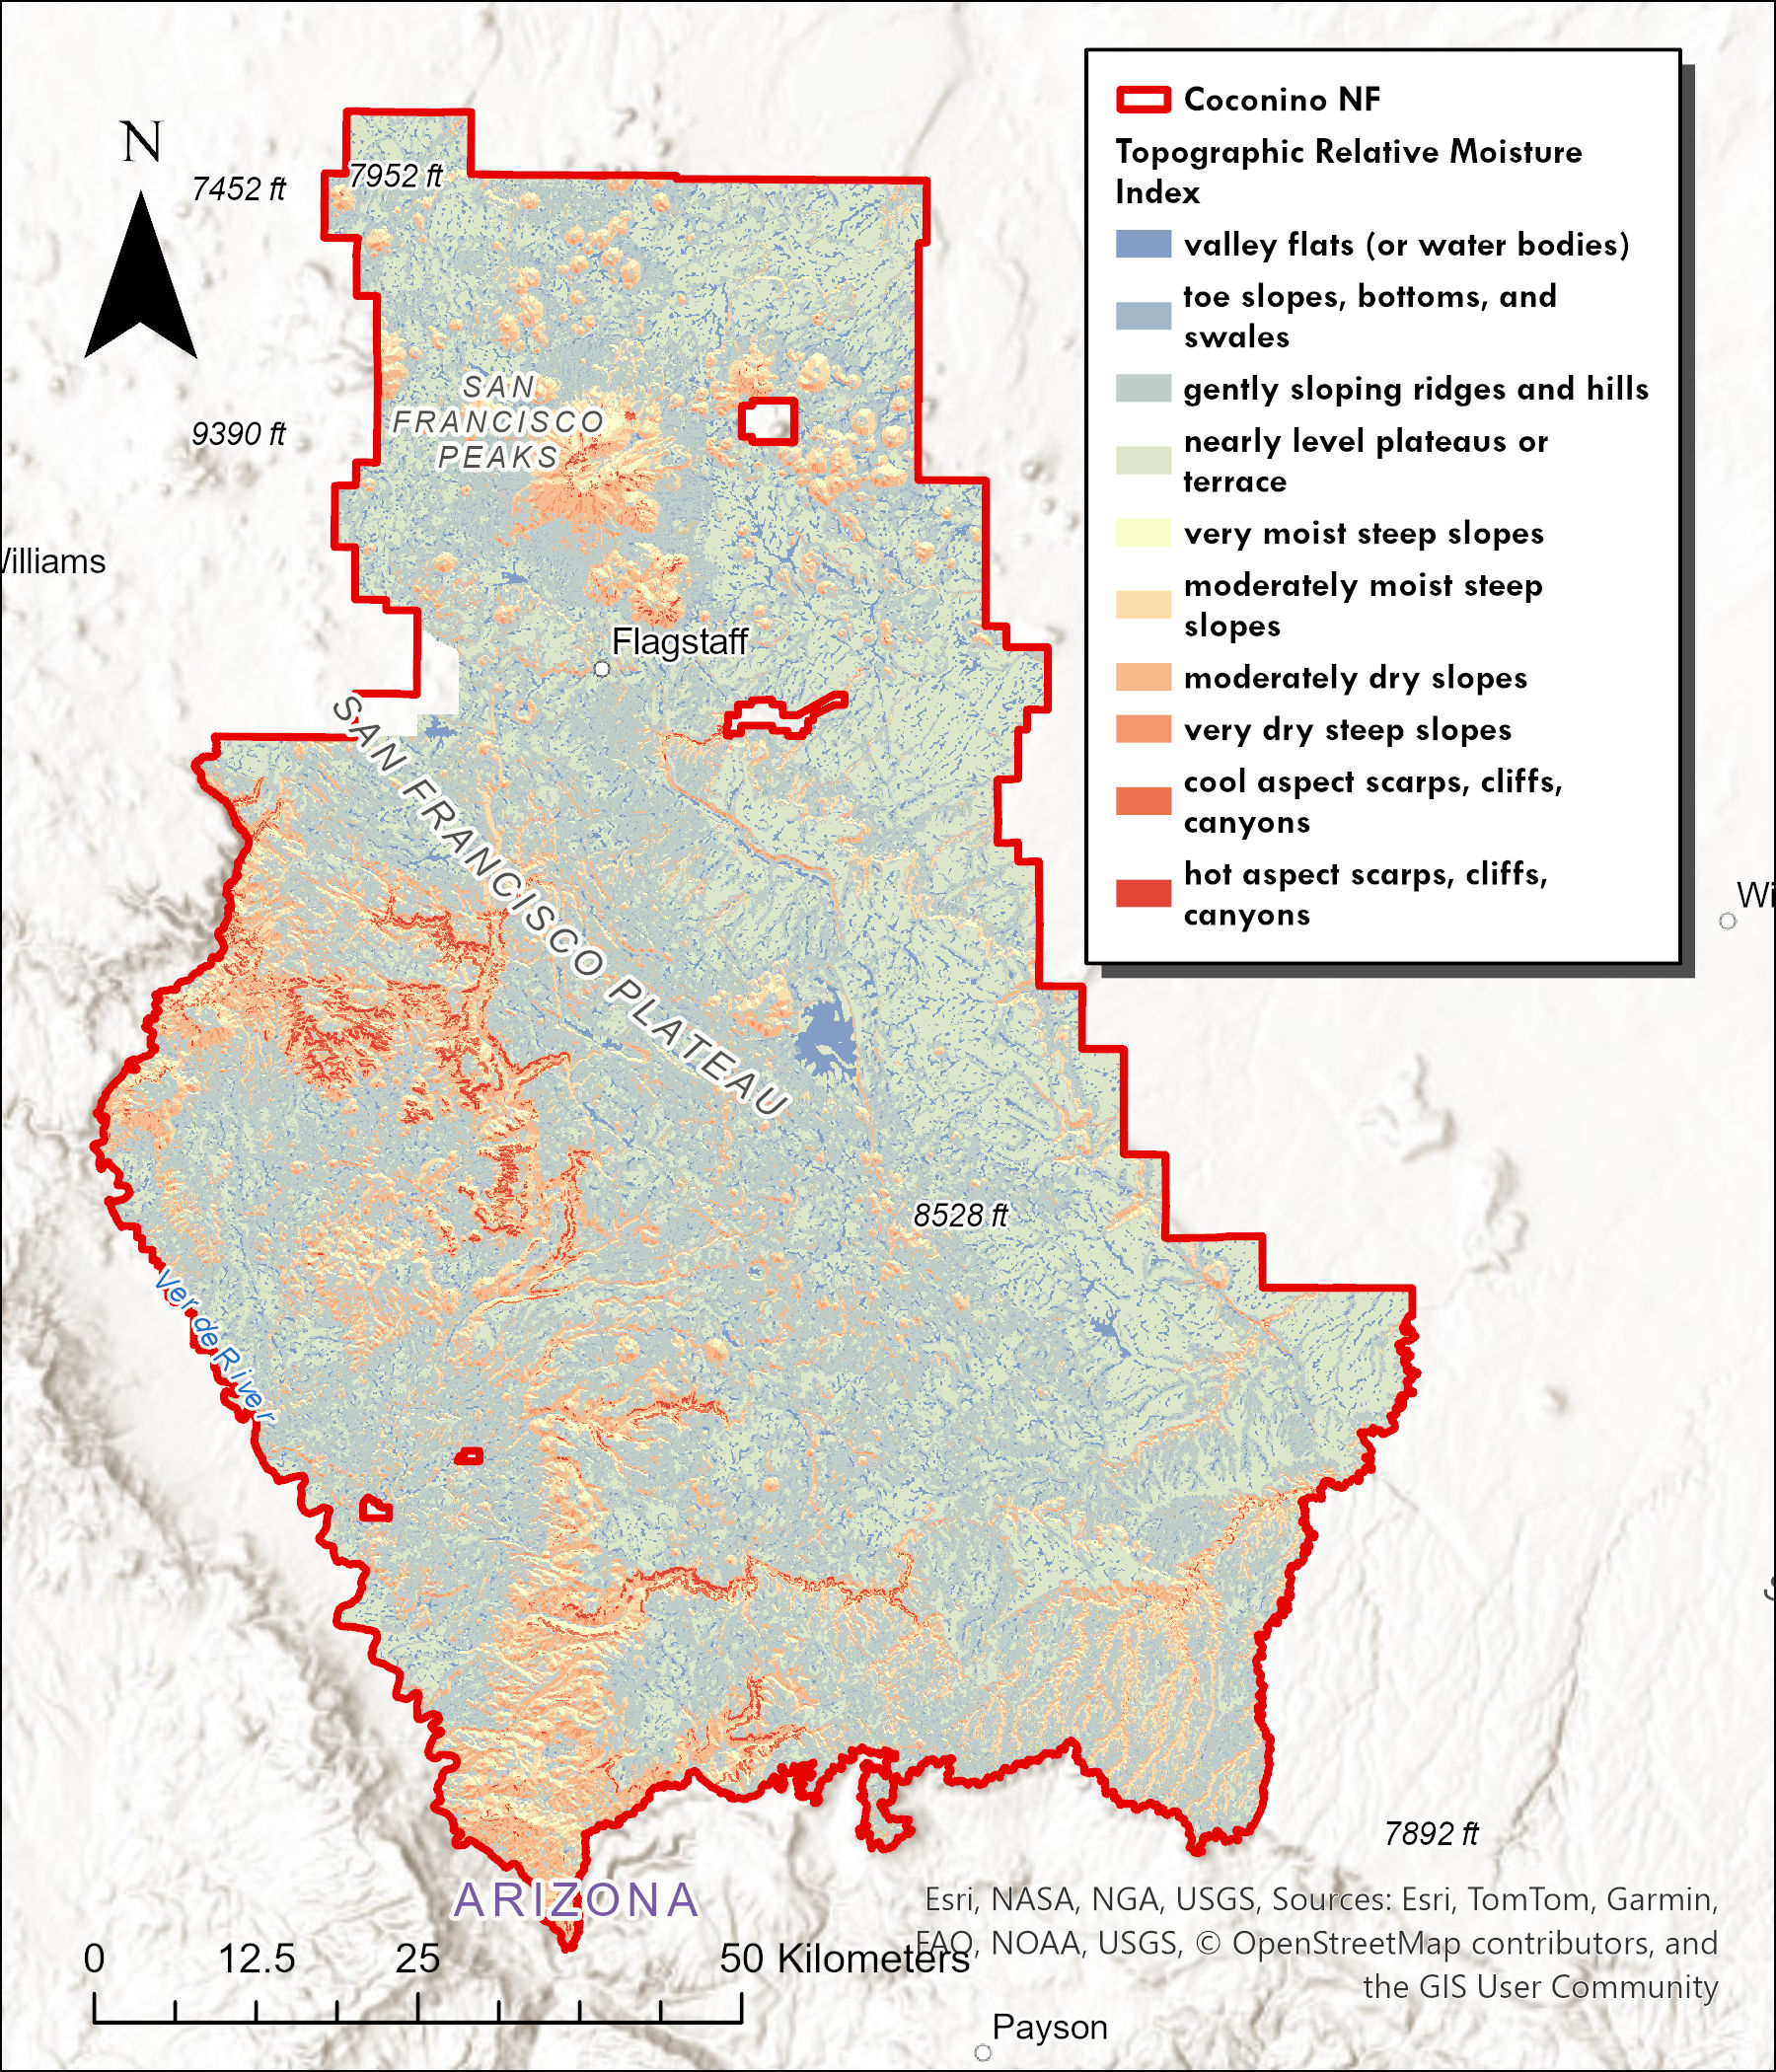
\includegraphics[keepaspectratio]{images/TRMI.jpg}}

}

\caption{Topographic Relative Moisture Index from the Southwest Regional
Gap Analysis (SWReGAP)}

\end{figure}%

\textbf{TO DO Replace image above with new manual TRMI}

\subsection{Basal Area}\label{basal-area}

We extracted basal area estimates from the TreeMap 2016
\citep{riley2022} CONUS dataset.

\begin{figure}[H]

{\centering \pandocbounded{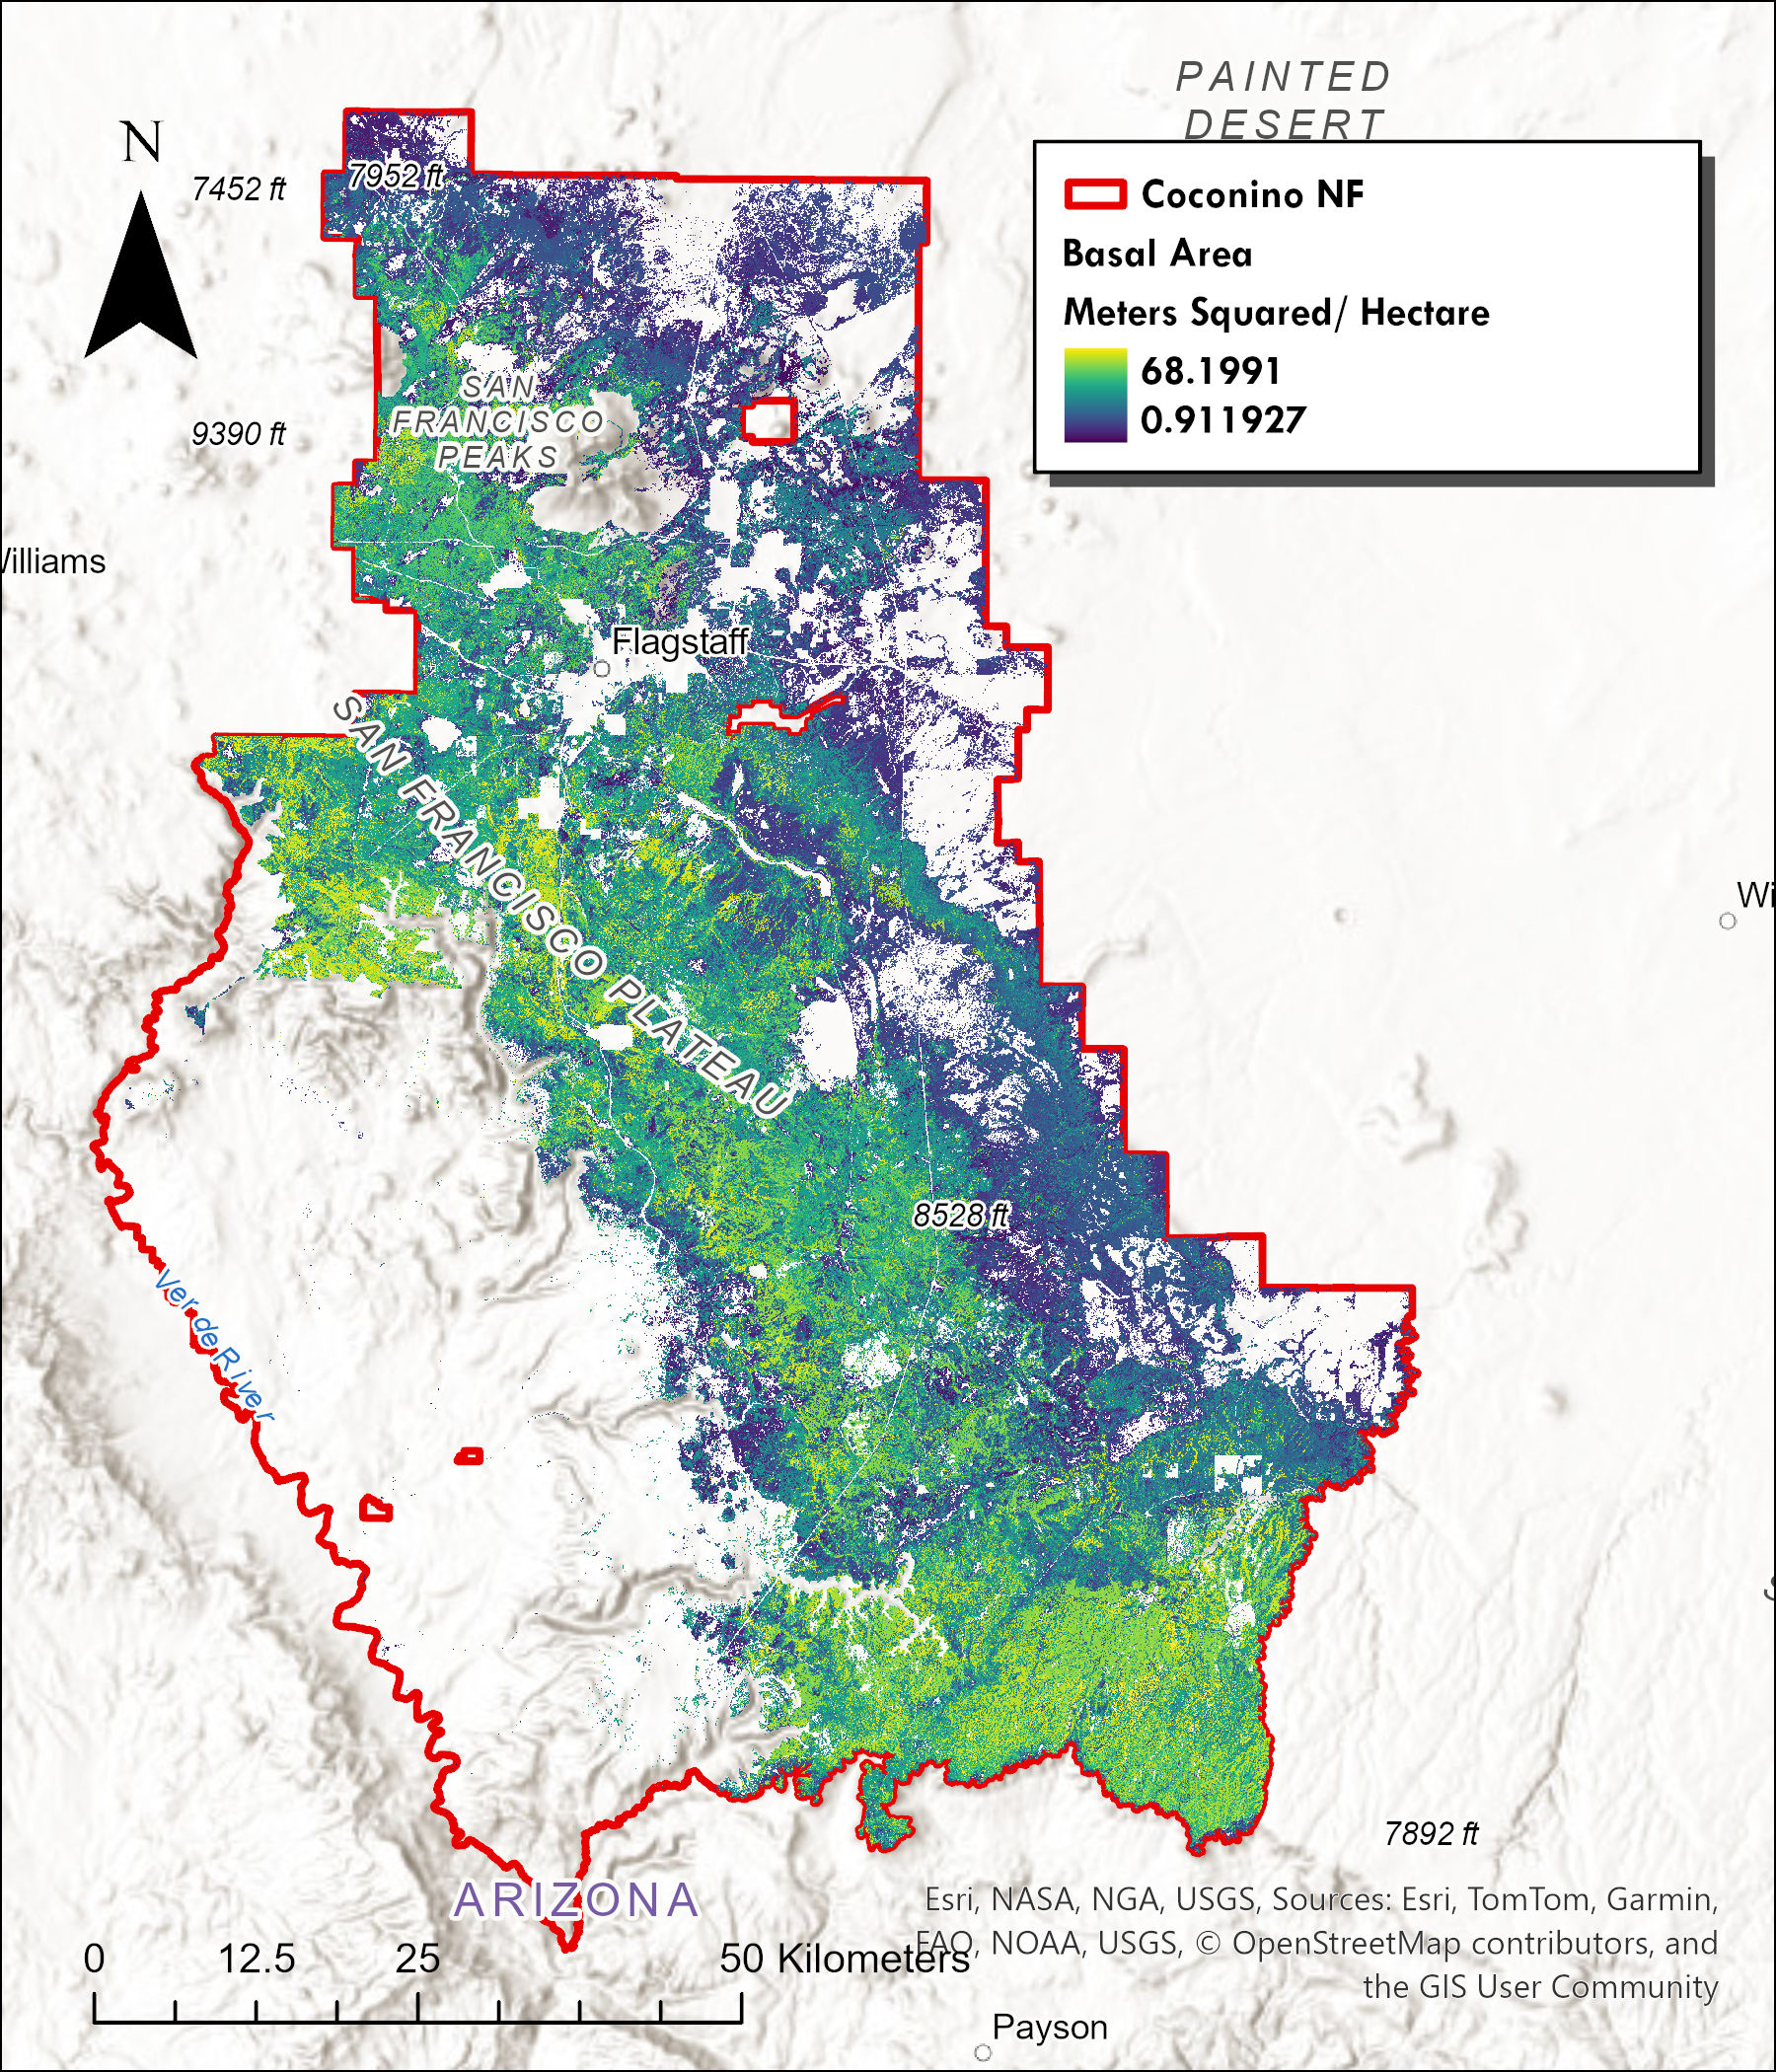
\includegraphics[keepaspectratio]{images/Basal_Area.jpg}}

}

\caption{Basal Area in cubic meters per hectare derived from the 2016
TreeMap dataset.}

\end{figure}%

\subsection{Snowfall Dominance}\label{snowfall-dominance}

Ask Patrick Broxton how it was calculated.

\begin{figure}[H]

{\centering \pandocbounded{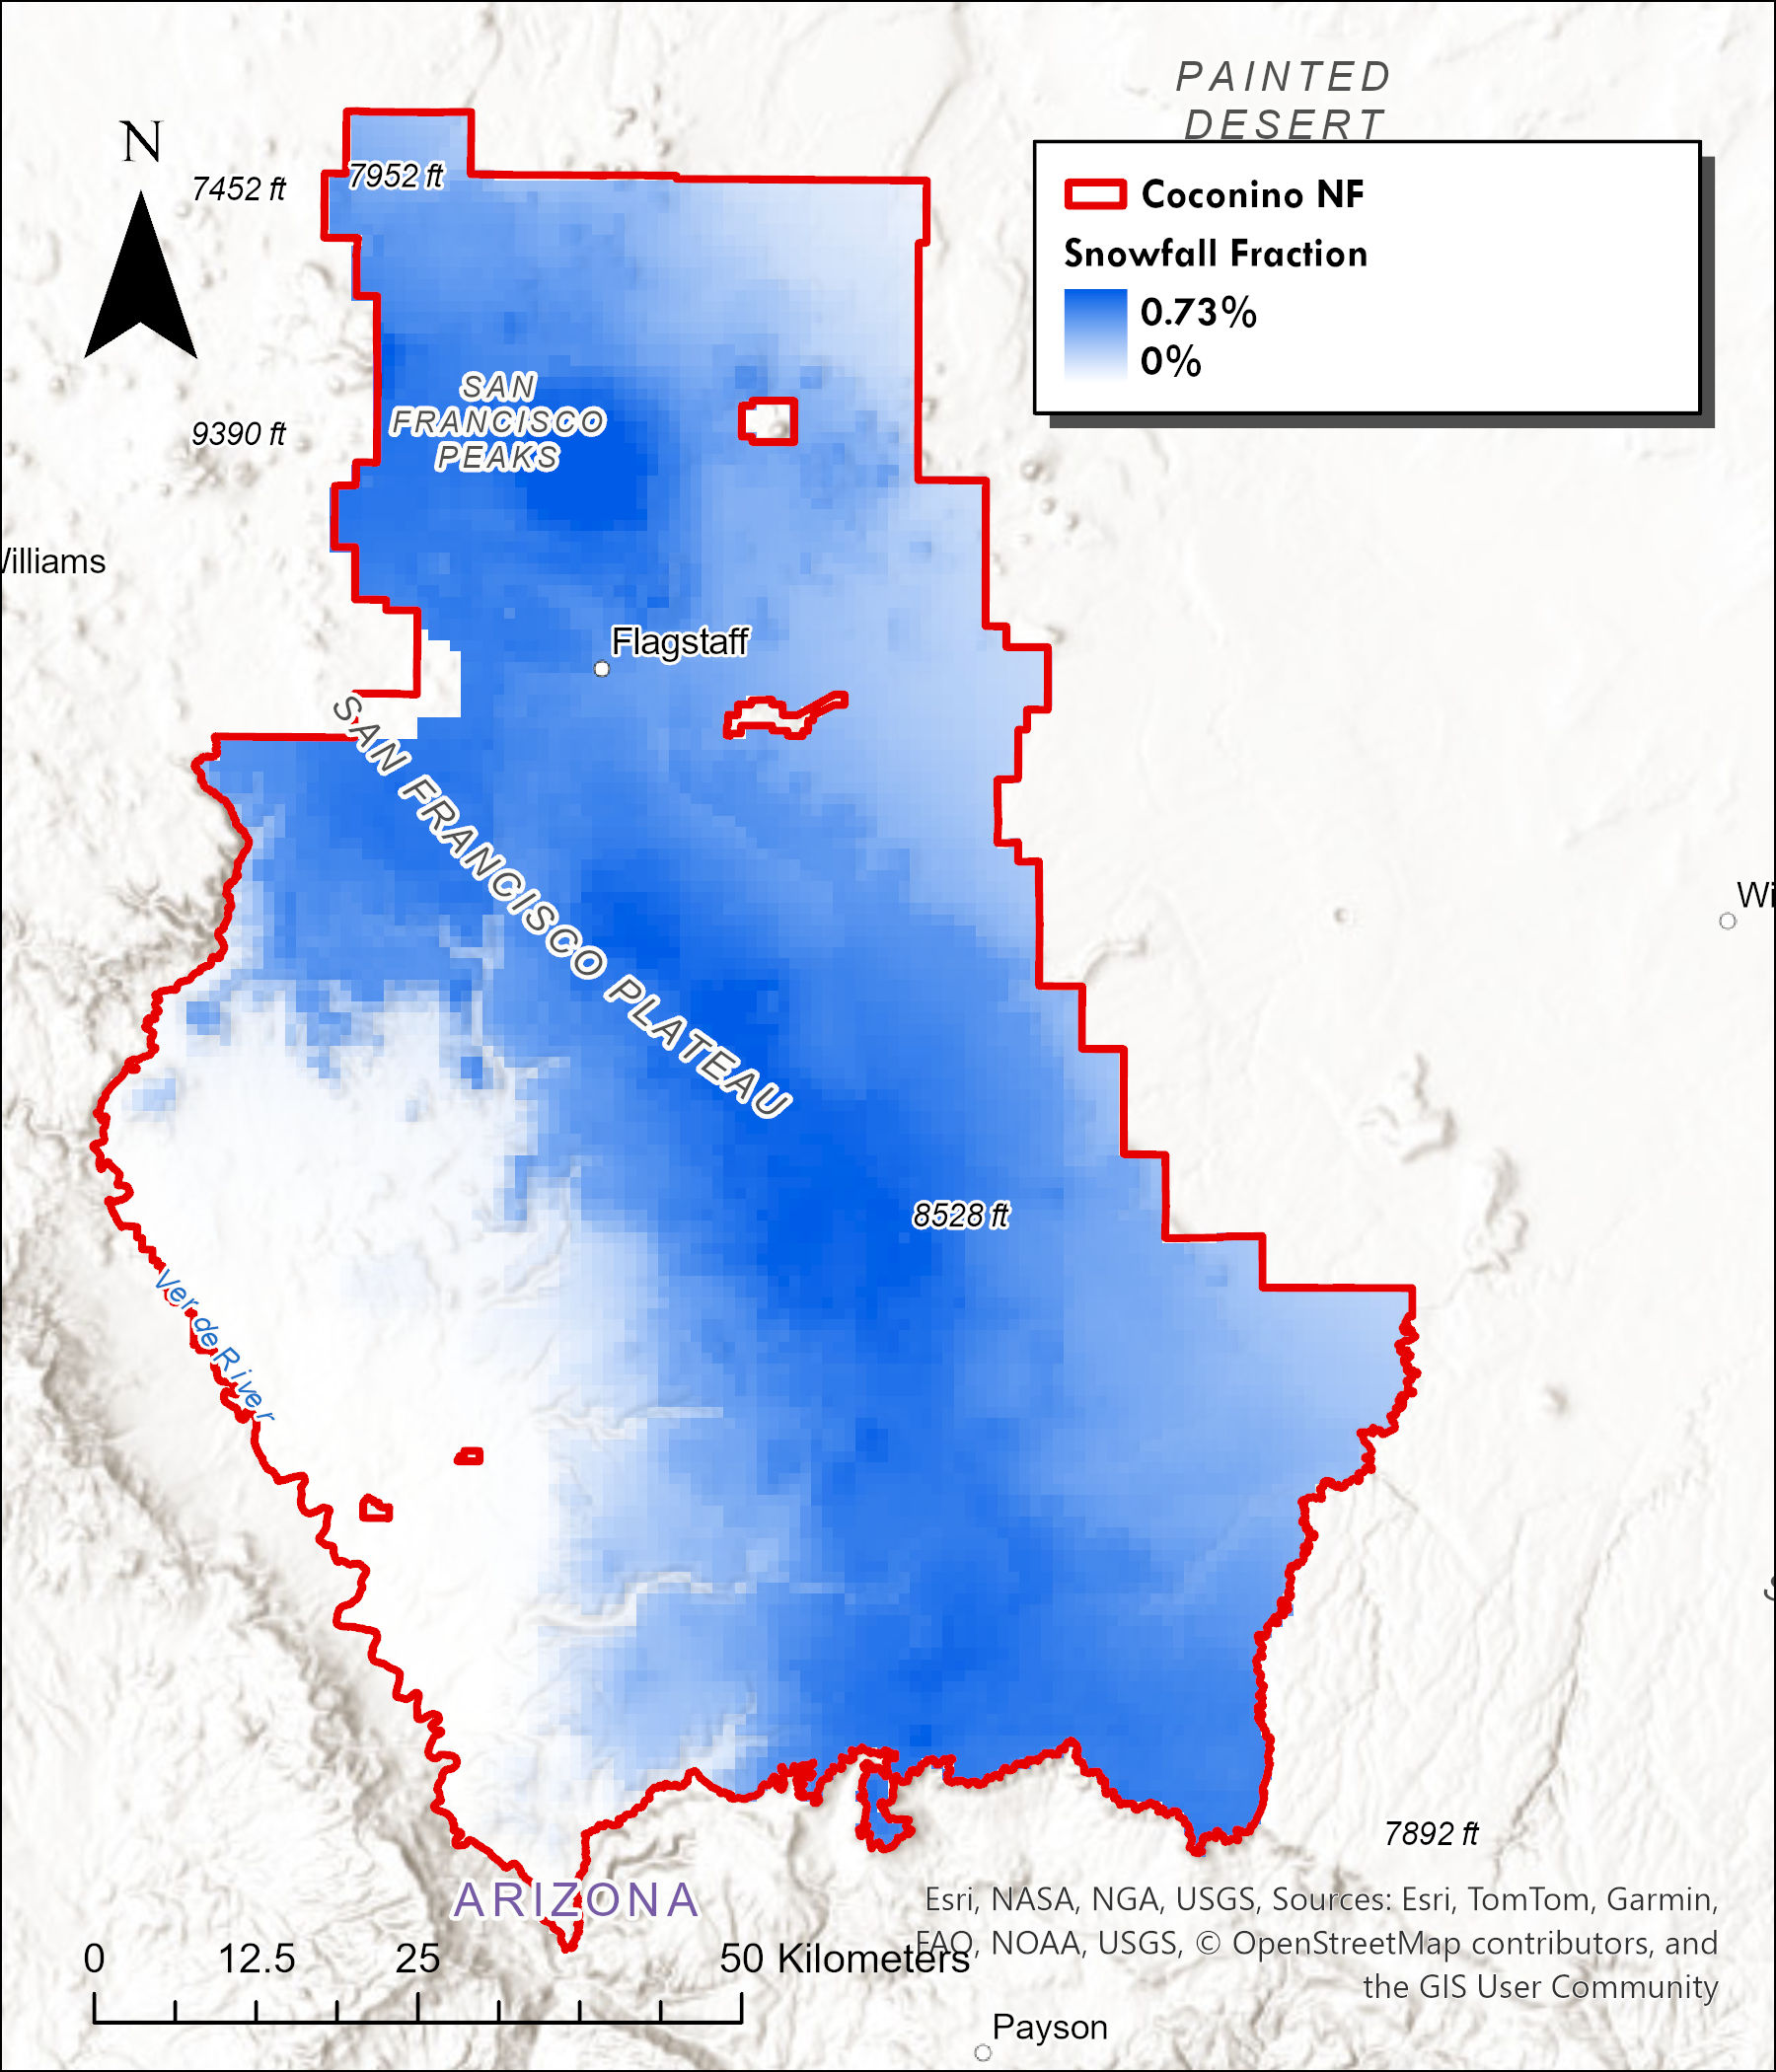
\includegraphics[keepaspectratio]{images/Snowfall Fraction.jpg}}

}

\caption{Percentage of Annual Precipitation that Falls as Snow}

\end{figure}%

\subsection{Mean Annual Precipitation}\label{mean-annual-precipitation}

Utilized AORC Retrospective forcing data for average water year (WY)
precipitation 1991 - 2020

\begin{figure}[H]

{\centering \pandocbounded{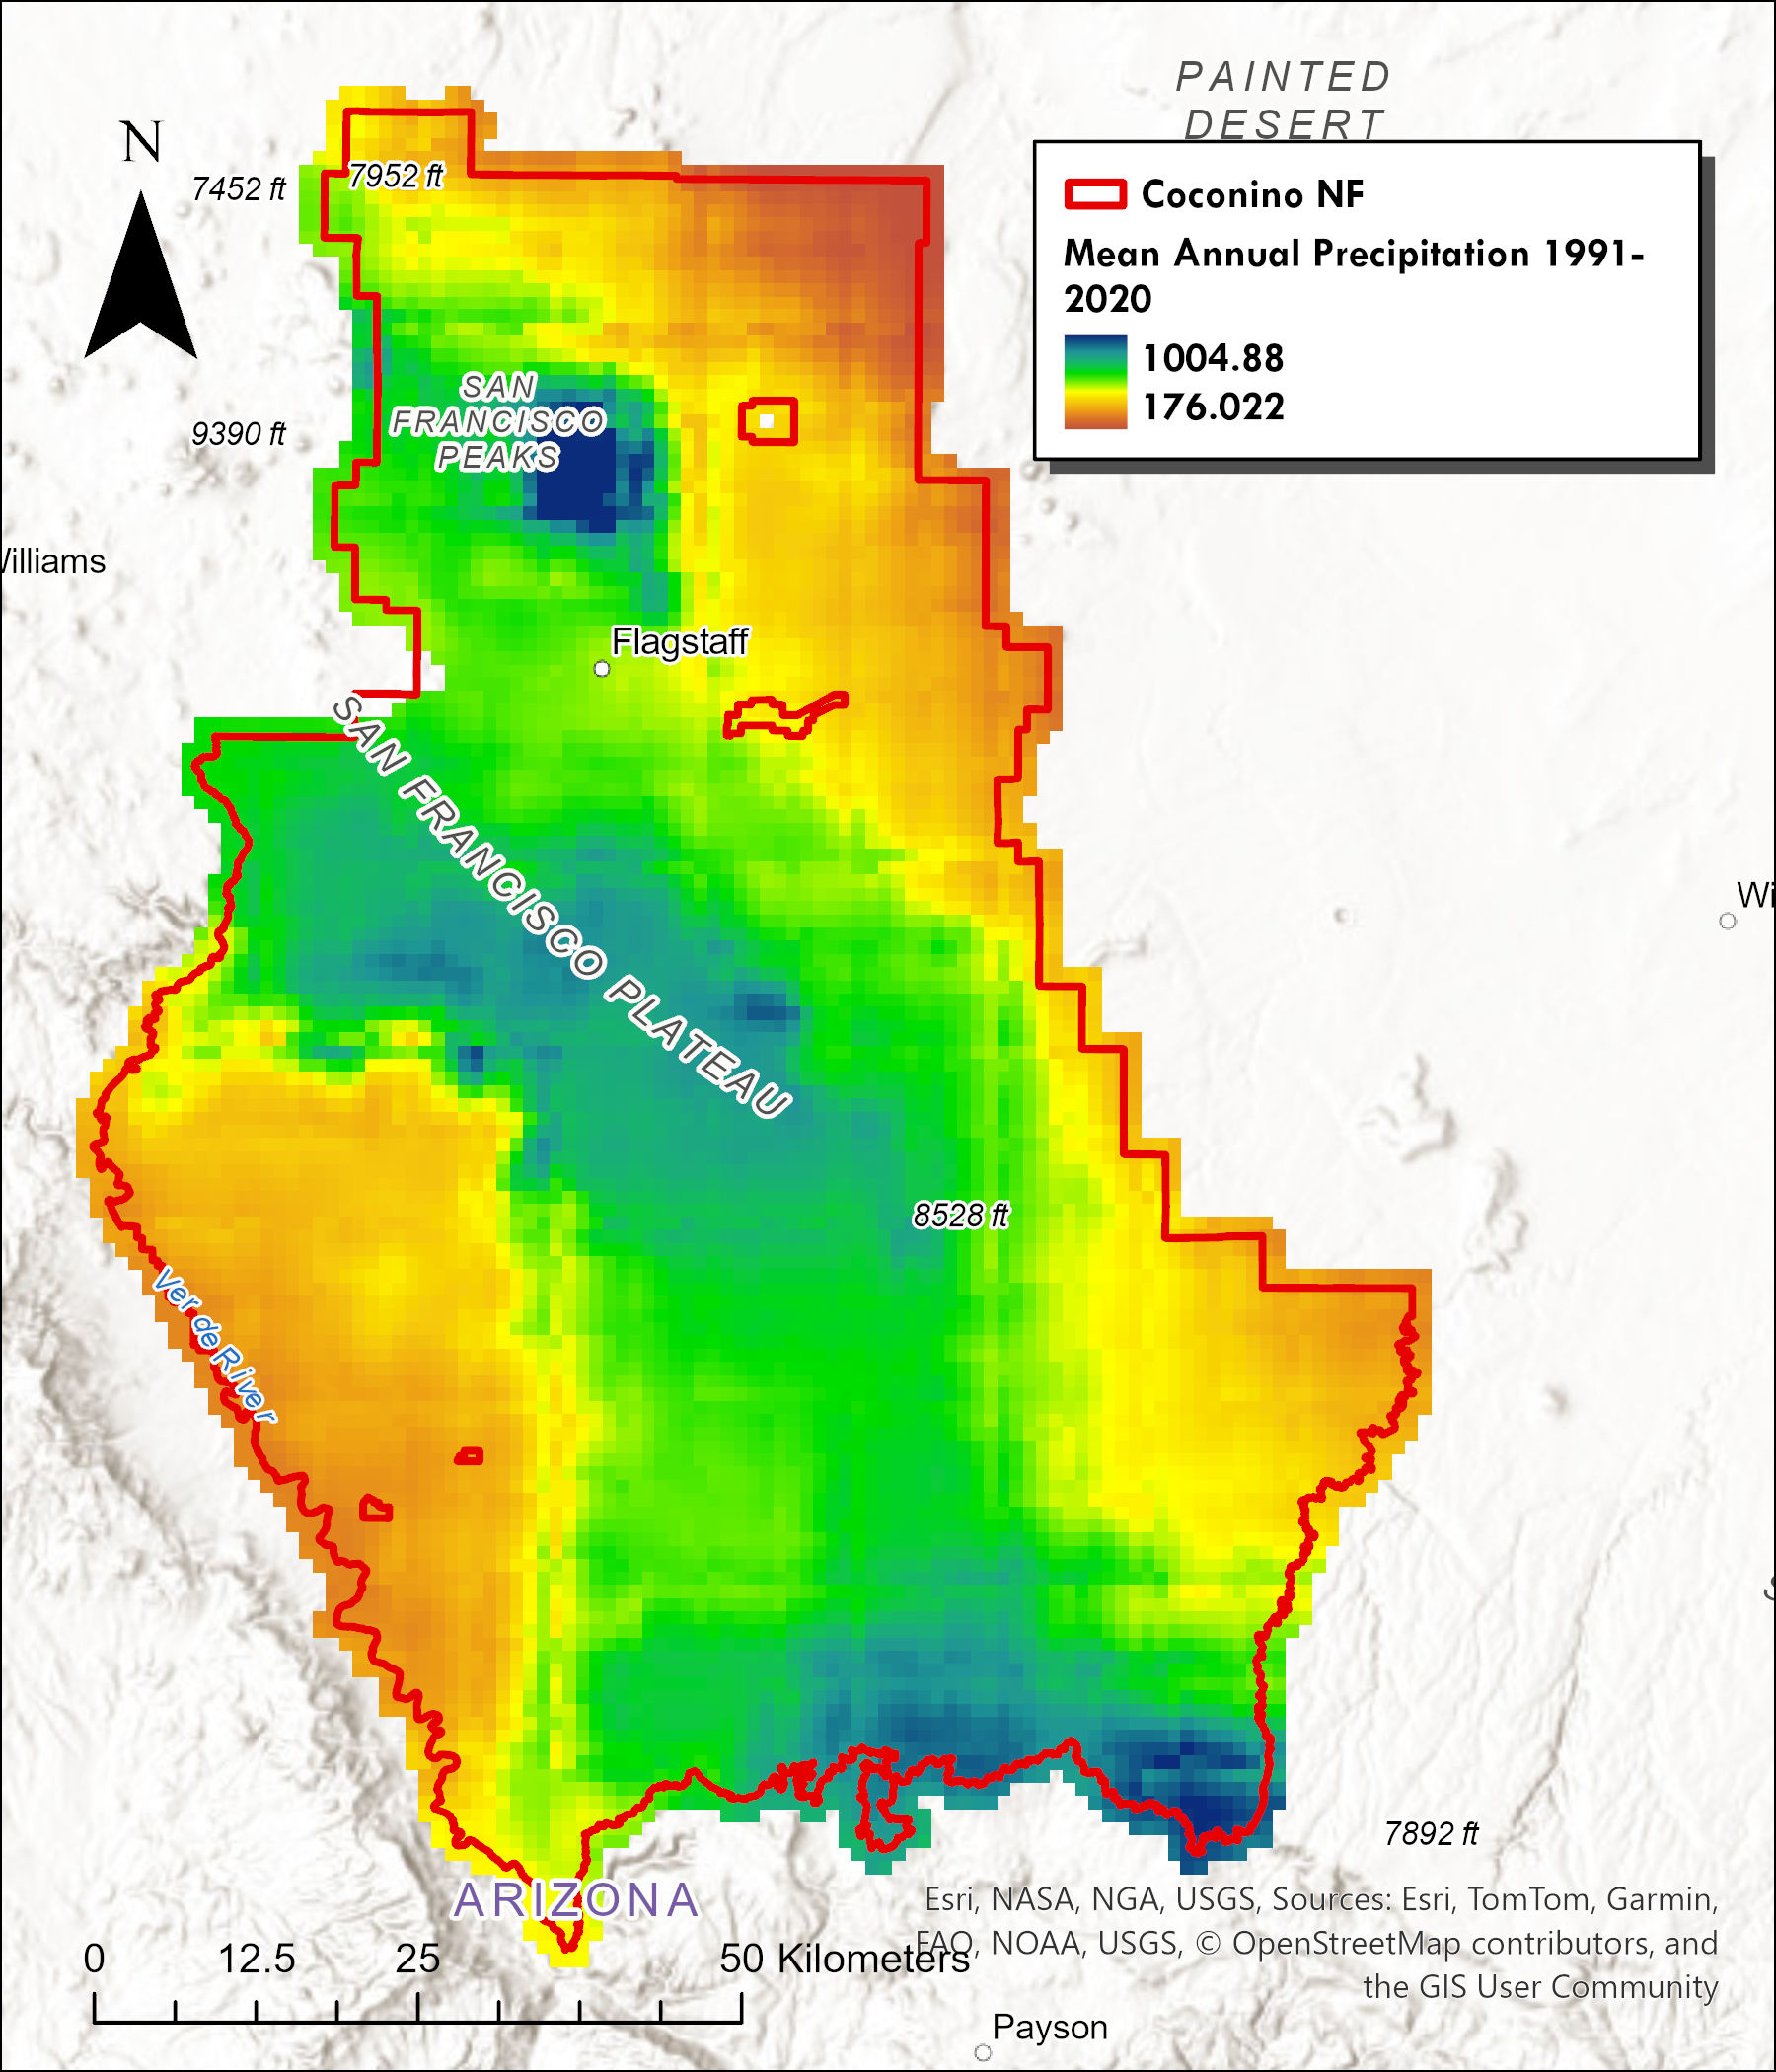
\includegraphics[keepaspectratio]{images/Mean_Annual_Precipitation.jpg}}

}

\caption{Mean Annual Precipitation for years 1991 - 2020}

\end{figure}%

\subsection{Subsurface Infiltration
Capacity}\label{subsurface-infiltration-capacity}

We utilized the Global Hydrological Maps of Permeability and Porosity
(GLHYMPS) to estimate subsurface infiltration capacity
\citep{gleeson2014}

\begin{figure}[H]

{\centering \pandocbounded{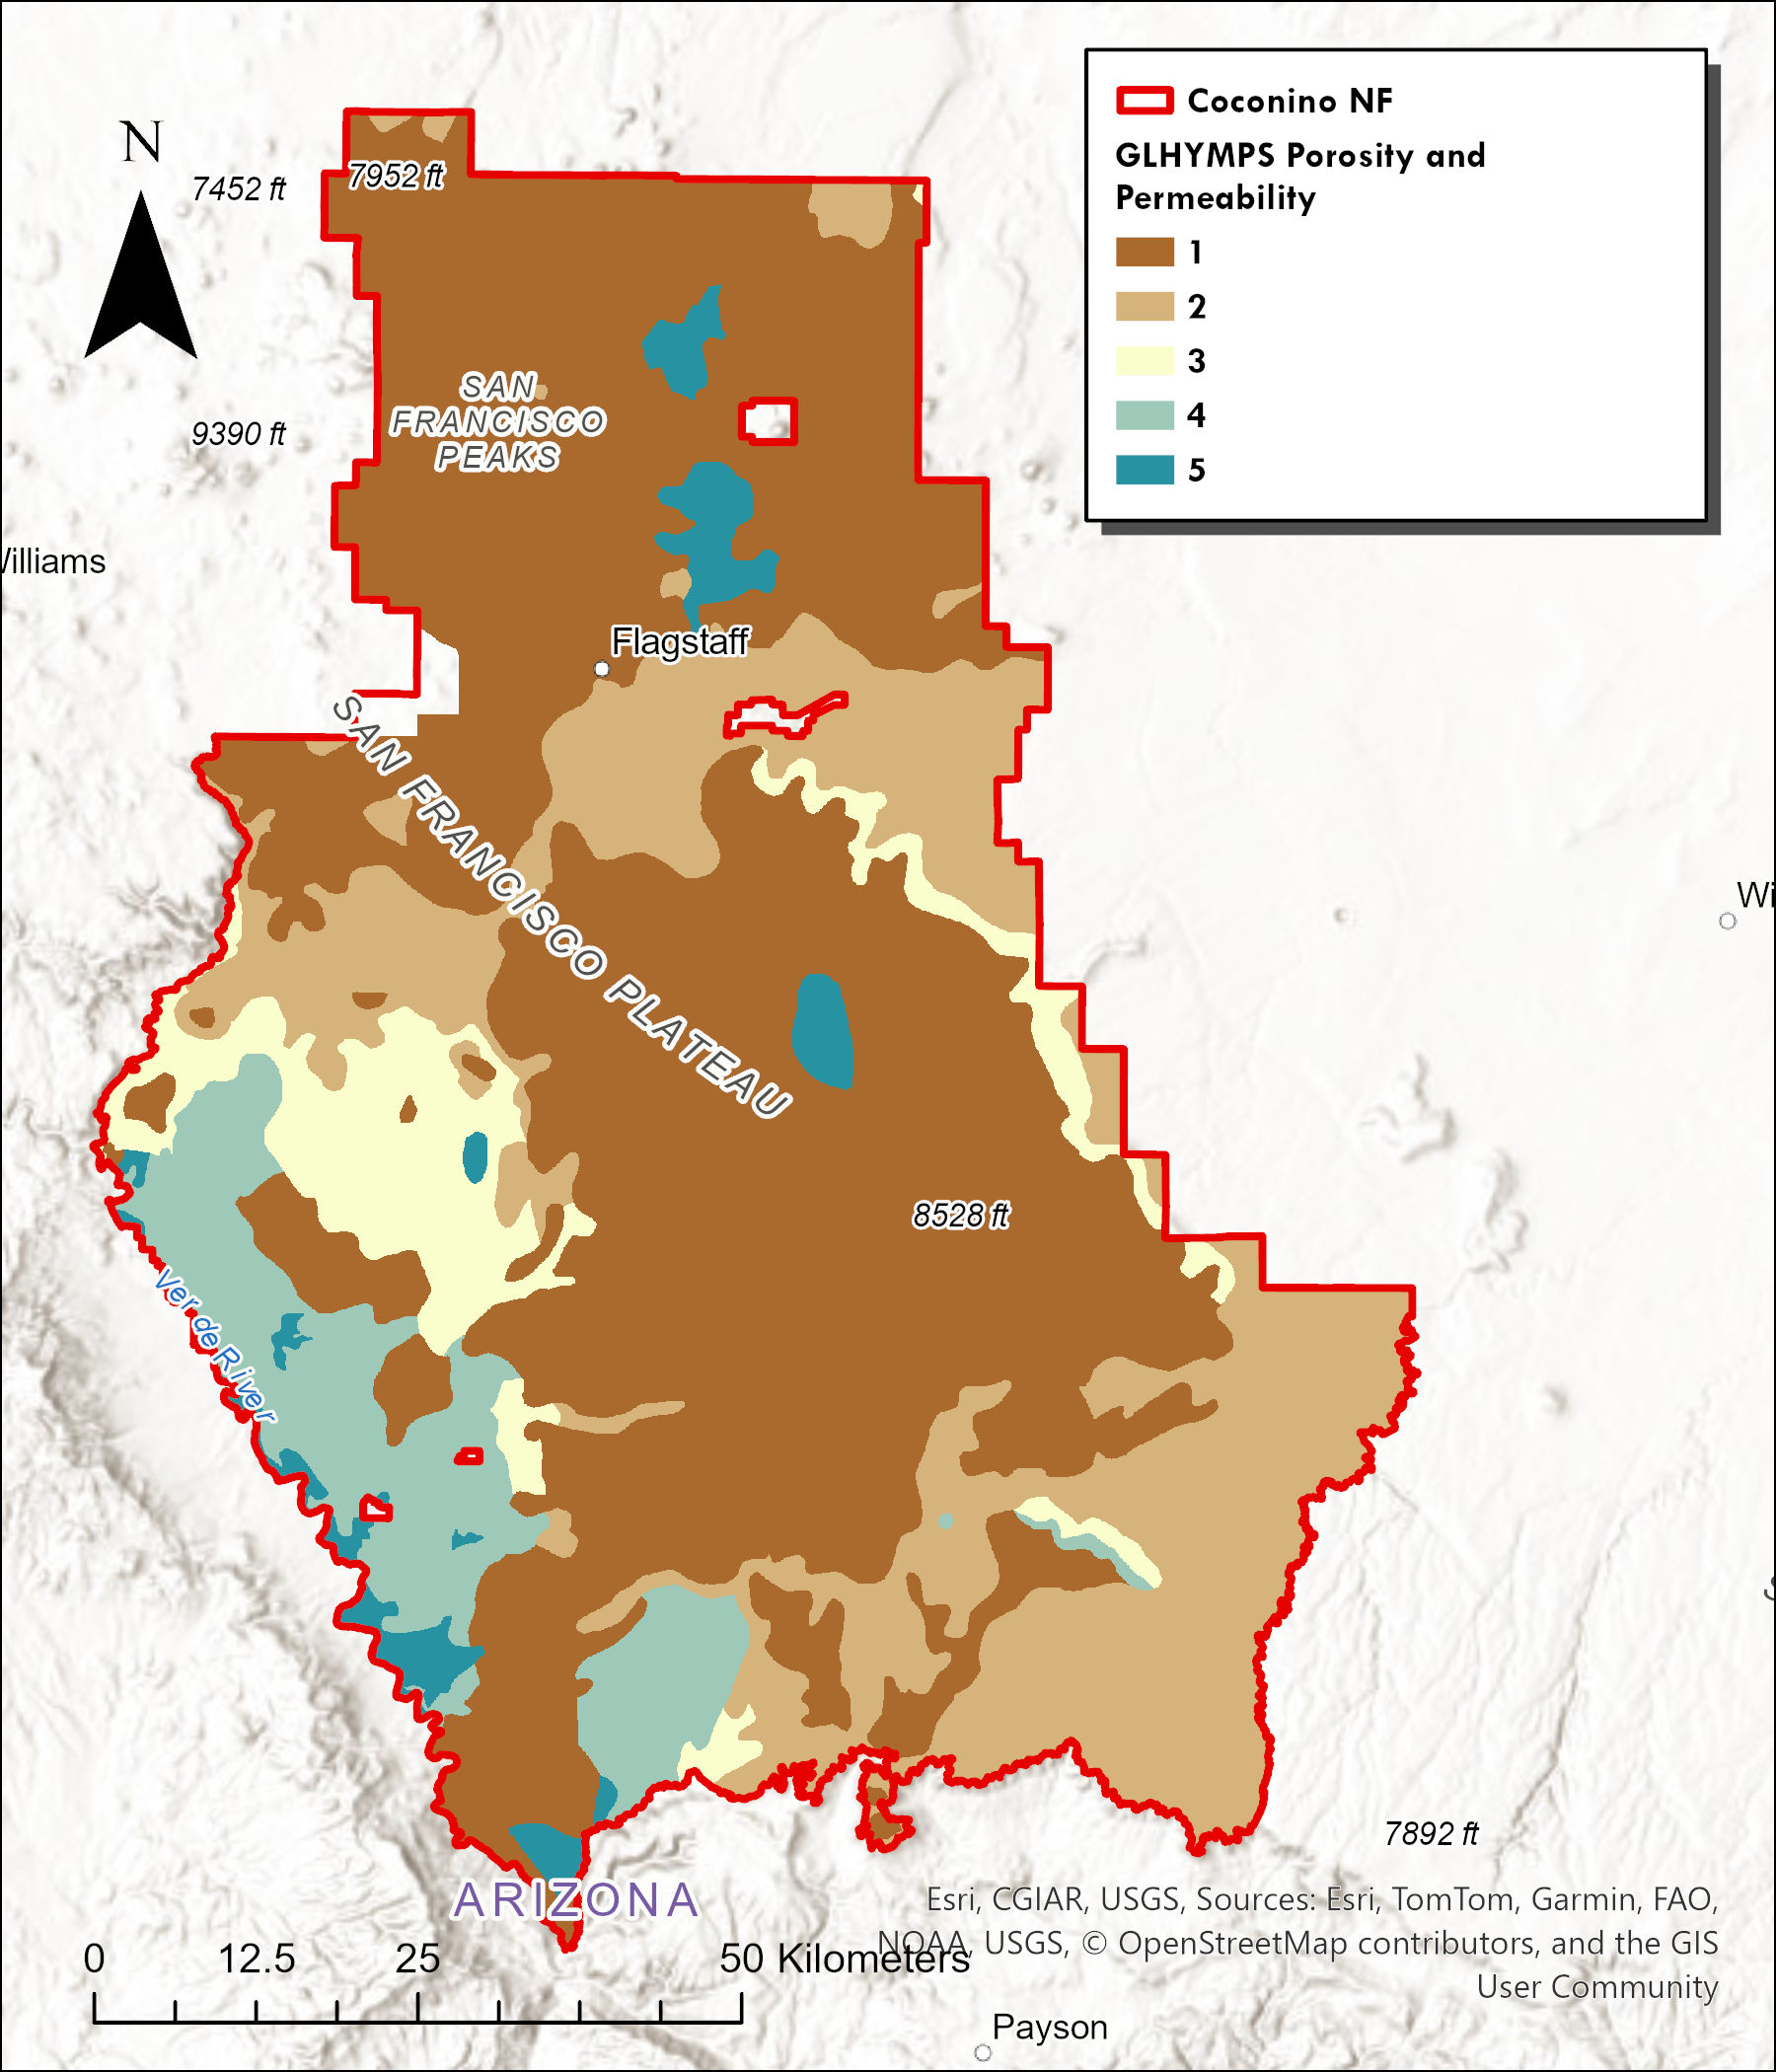
\includegraphics[keepaspectratio]{images/GLHYMPS.jpg}}

}

\caption{Subsurface Infiltration Capacity, a combination of Permeability
and Porosity values from the GLHYMPS dataset (Gleeson et al., 2014).
Higher values (cooler colors) indicate higher infiltration capacity,
while browner colors and lower values indicate lower infiltration
capacity. Keep in mind this does not consider secondary or tertiary
permeability or porosity due to faults, fractures, caves, and conduits.}

\end{figure}%

\subsection{Soil Hydrologic Type}\label{soil-hydrologic-type}

\textbf{TO DO} \textbf{\emph{eventually we should replace Hydrologic
Soil Type with a Soil Infiltration Index composed of Soil Saturated Ksat
(weight = 0.5), Depth to bedrock (weight = 0.3) and Drainage Class
(0.2), after normalizing each variable we can combine them into a matrix
which will provide a better weighting scheme than just applying values
0-10 to hydrologic class.}}

Hydrologic Soil Type data from gNATSGO was used to estimate the soil's
ability to infiltrate water. Four soil types were identified within the
study area (fig soil) which were subsequently reclassified from 4 - 10
according to the tablex below.

\begin{longtable}[]{@{}
  >{\raggedright\arraybackslash}p{(\linewidth - 4\tabcolsep) * \real{0.2917}}
  >{\raggedright\arraybackslash}p{(\linewidth - 4\tabcolsep) * \real{0.4583}}
  >{\raggedright\arraybackslash}p{(\linewidth - 4\tabcolsep) * \real{0.2500}}@{}}
\toprule\noalign{}
\begin{minipage}[b]{\linewidth}\raggedright
Hydrologic Soil Type
\end{minipage} & \begin{minipage}[b]{\linewidth}\raggedright
Description
\end{minipage} & \begin{minipage}[b]{\linewidth}\raggedright
Suitability Class
\end{minipage} \\
\midrule\noalign{}
\endhead
\bottomrule\noalign{}
\endlastfoot
A & Group A soils consist of deep, well drained sands or gravelly sands
with high infiltration and low runoff rates. & 10 \\
B & Group B soils consist of deep well drained soils with a moderately
fine to moderately coarse texture and a moderate rate of infiltration
and runoff. & 8 \\
C & Group C consists of soils with a layer that impedes the downward
movement of water or fine textured soils and a slow rate of
infiltration. & 6 \\
D & Group D consists of soils with a very slow infiltration rate and
high runoff potential. This group is composed of clays that have a high
shrink-swell potential, soils with a high water table, soils that have a
clay pan or clay layer at or near the surface, and soils that are
shallow over nearly impervious material. & 4 \\
\end{longtable}

\begin{figure}[H]

{\centering \pandocbounded{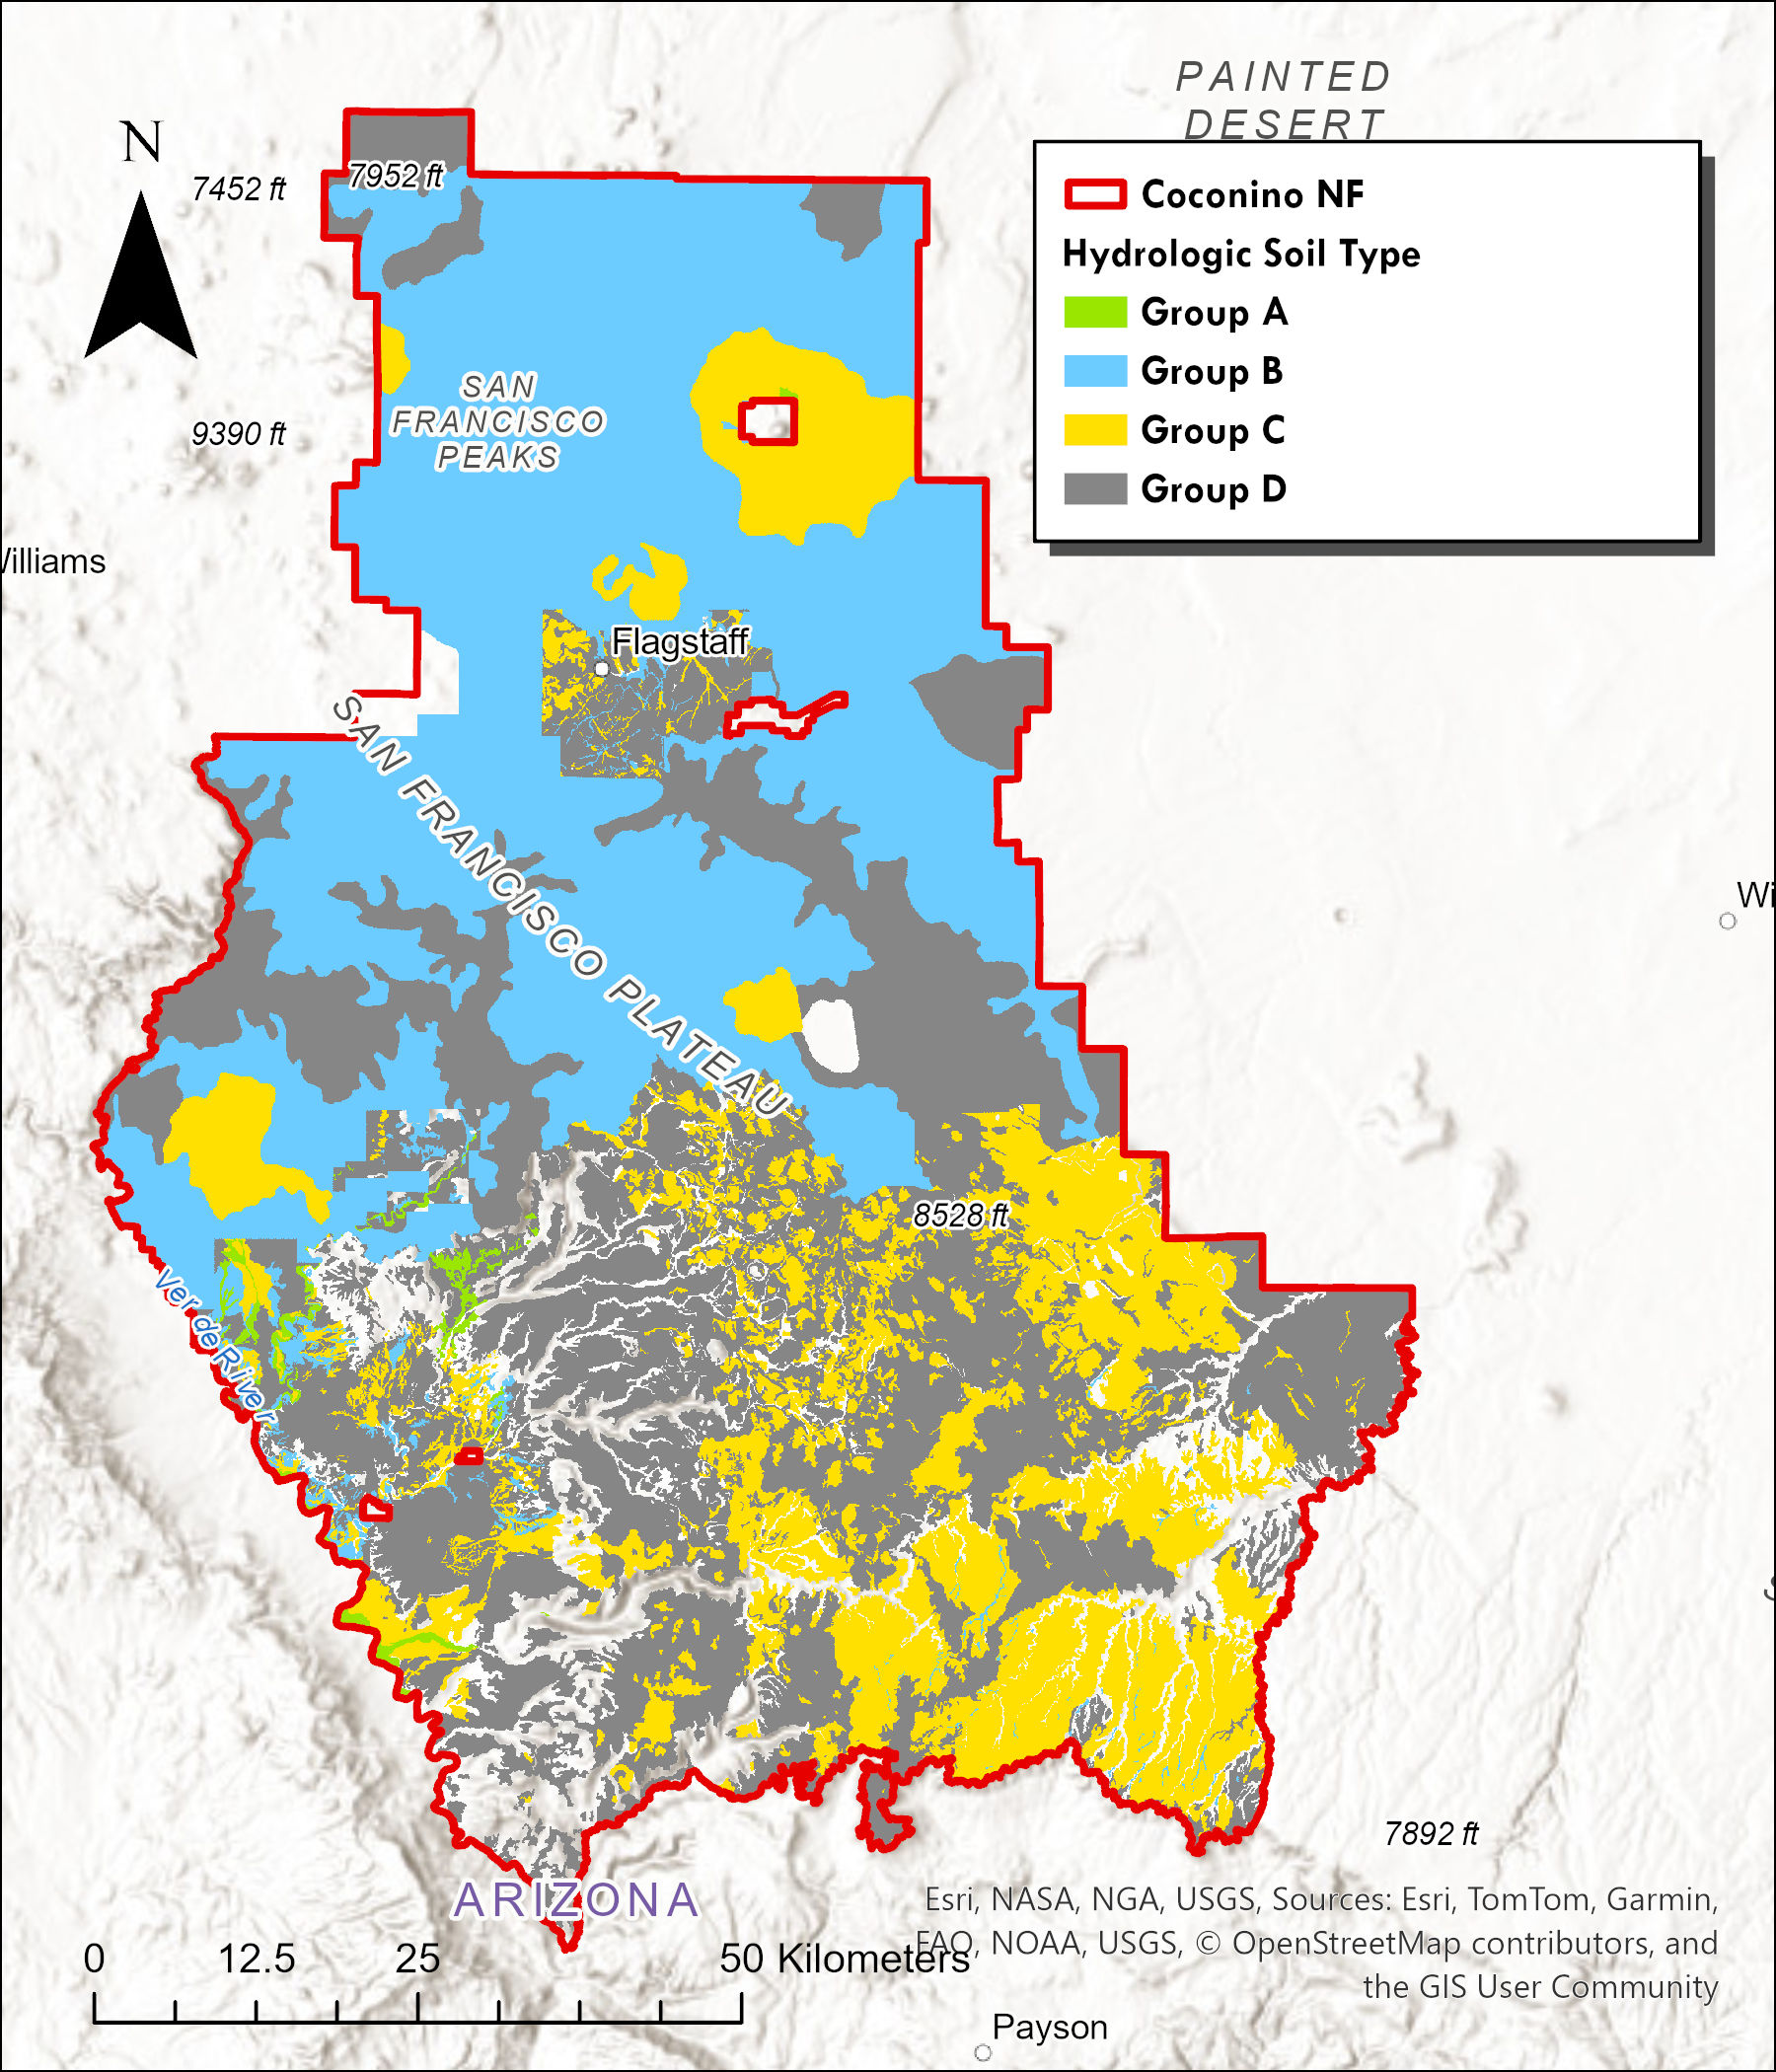
\includegraphics[keepaspectratio]{images/Hydrologic_soil_type.jpg}}

}

\caption{Hydrologic Soil Type from gNATSGO.}

\end{figure}%

\subsection{Canopy Cover}\label{canopy-cover}

Reconstructions of pre-settlement ponderosa pine forests have found a
range of canopy covers between 10\% and 22\%, with a median of 16.7\%
canopy cover\citep{huffman2012}. However, UAV-analyses of snow pack in
thinned and un-thinned ponderosa pine forests within the study area
found that canopy cover is highly predictive of snow persistence and
that 24 - 35\% canopy cover was optimal for maintaining snowpack.
\citep{donager2021, sankey_multi-scale_2015, belmonte_uav-based_2021}.
However a reduction of 20\% canopy cover is necessary to reduce ET and
enhance water yield \citep{adams_ecohydrological_2012} . However
thinning treatments are costly and several studies have shown that
thinning treatments can lead to soil compaction and reduced infiltration
\citep{moreno2016}. Maximum suitability, then would be the areas with
29-42\% canopy cover where the a 20\% reduction would result in forests
with canopy covers of between 24\% and 35\%. Higher forest covers could
also be suitable but would require more thinning and likely more soil
compaction. We set the minimum suitability at 12\% canopy cover, since a
minimum 20\% reduction would result in canopy cover of about 10\% the
low end of the canopy cover found in pre-settlement forests
\citep{huffman2012}.

Canopy Cover was obtained from the 2021 National Land Cover Database ,
which provides an estimate of Total Canopy Cover (figure x). Canopy
cover values ranged from 0\% - 86\%, the canopy cover data was
reclassified using a Gaussian (parabolic) function centering on 35\%.
The maximum threshold was left at 86\%, while the minimum threshold was
set to 20\%, with a spread of 0.0085. In this way, regions with canopy
cover approaching 35\% were classified as 10, and suitability
classification decreased continuously as canopy cover diverged from th
35\% target value.

\begin{figure}[H]

{\centering \pandocbounded{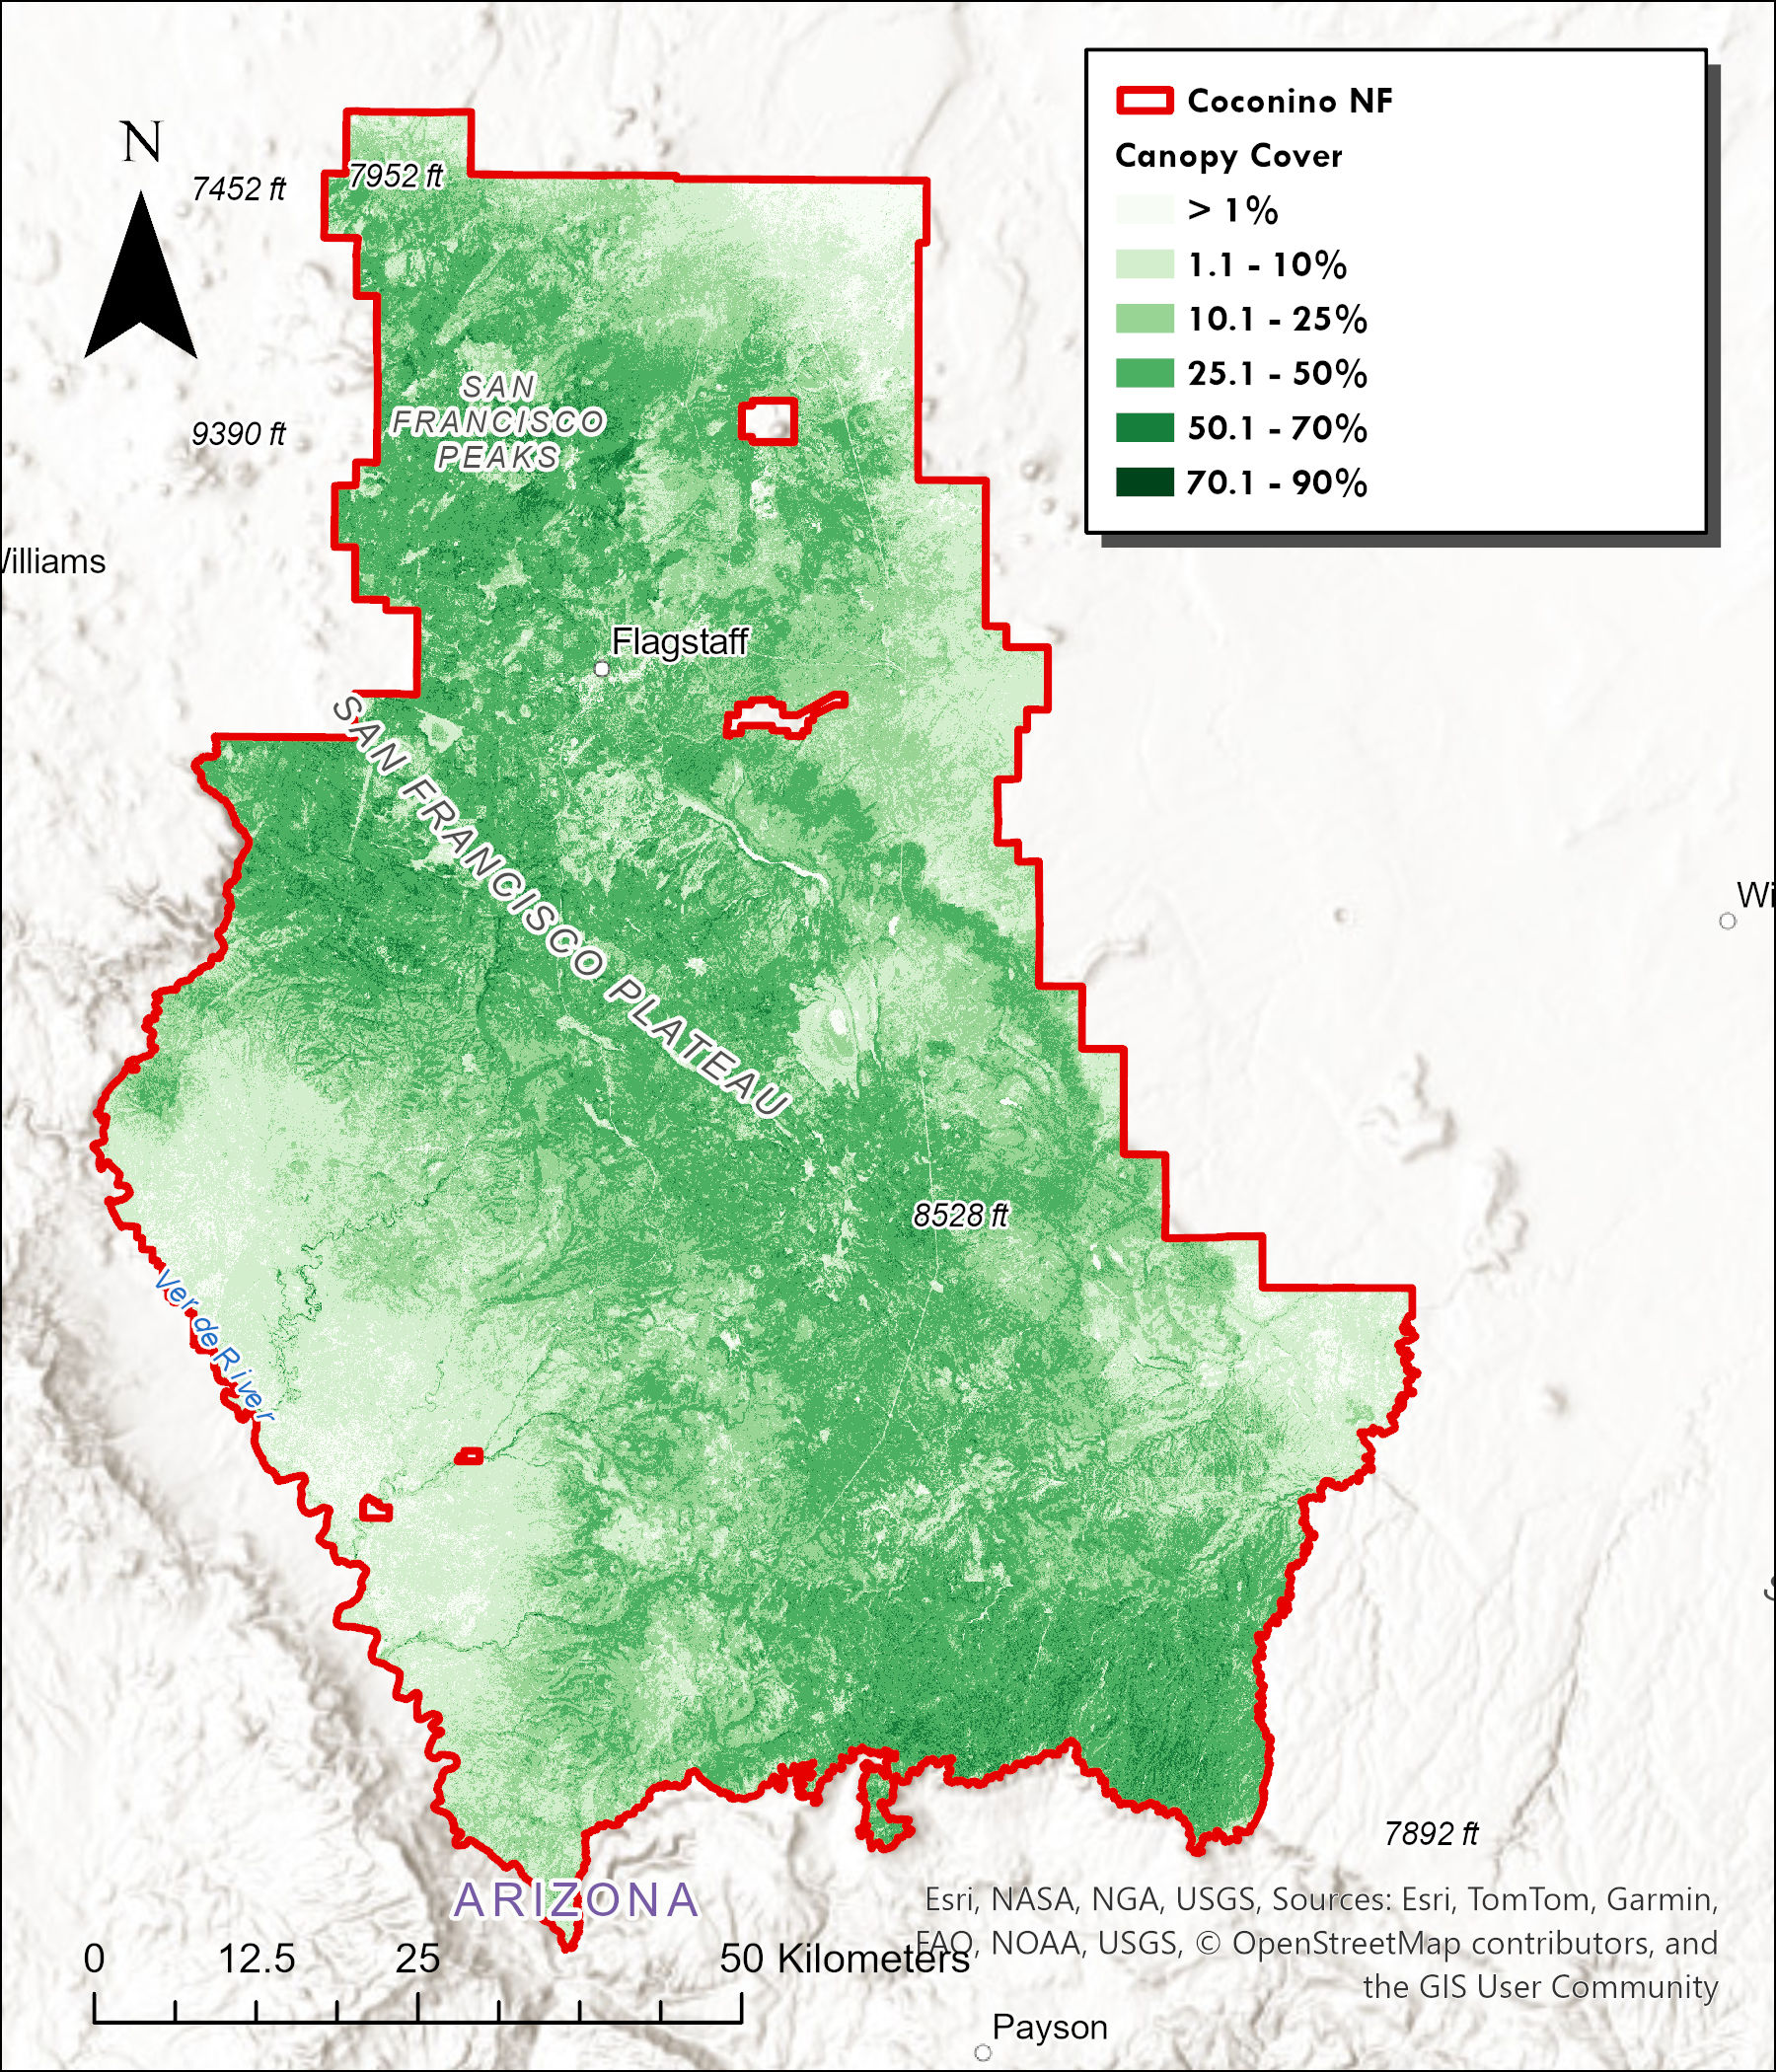
\includegraphics[keepaspectratio]{images/Canopy_Cover.jpg}}

}

\caption{Canopy Cover derived from the NLCD 2021}

\end{figure}%

\section{Weighting}\label{weighting}

Pairwise comparisons between each variable were made using the
\href{https://www.inowas.com/tools/t05-gis-mcda/}{INOWAS GIS MCDA tool}.
The pairwise comparisons were The resulting weight schema is presented
in Table 1. The weighting had a consistency ratio (CR) of 0.031, values
less than 0.1 are considered consistent.

\section{Model}\label{model}

\begin{figure}[H]

{\centering \pandocbounded{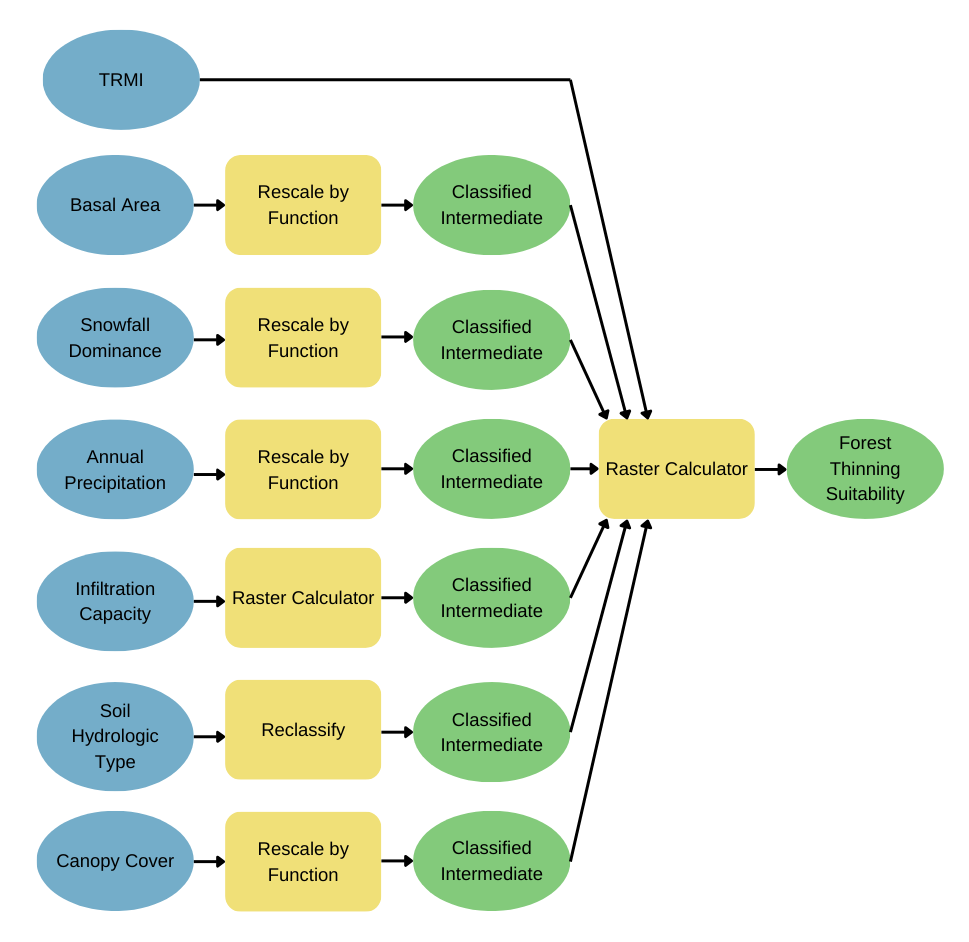
\includegraphics[keepaspectratio]{images/Model_Builder_new.png}}

}

\caption{Diagram of the suitability model workflow. Input data layers,
such as TRMI are shown in blue ovals, processing steps in yellow
rectangles, and computed data layers in green ovals..}

\end{figure}%

Results

The total study area was XXXXXX ha. The evaluated study area after masks
were applied excluding protected areas, incompatible land use/cover
types, and areas receving less than 500mm of maximum precipitation
(1991-2020) was 480,000 ha. About 95,000 ha (19.8\%) of the areas has
suitability values of 5 or greater, about 12,000 ha (2.5\%) have
suitability values of 6 or greater, and 65 ha with suitability values
greater than 7. Leaving about 384,000 ha (77\%) with suitability scores
less than 5. Importantly, while forest thinning in regions where the
suitability score is \textless5 is less likely to enhance aquifer
recharge, this does not mean that thinning will not enhance aquifer
recharge. Conversely areas may be deemed suitable by this analysis but
may be unsuitable with other policy or feasibility concerns are
considered.

\begin{figure}[H]

{\centering \pandocbounded{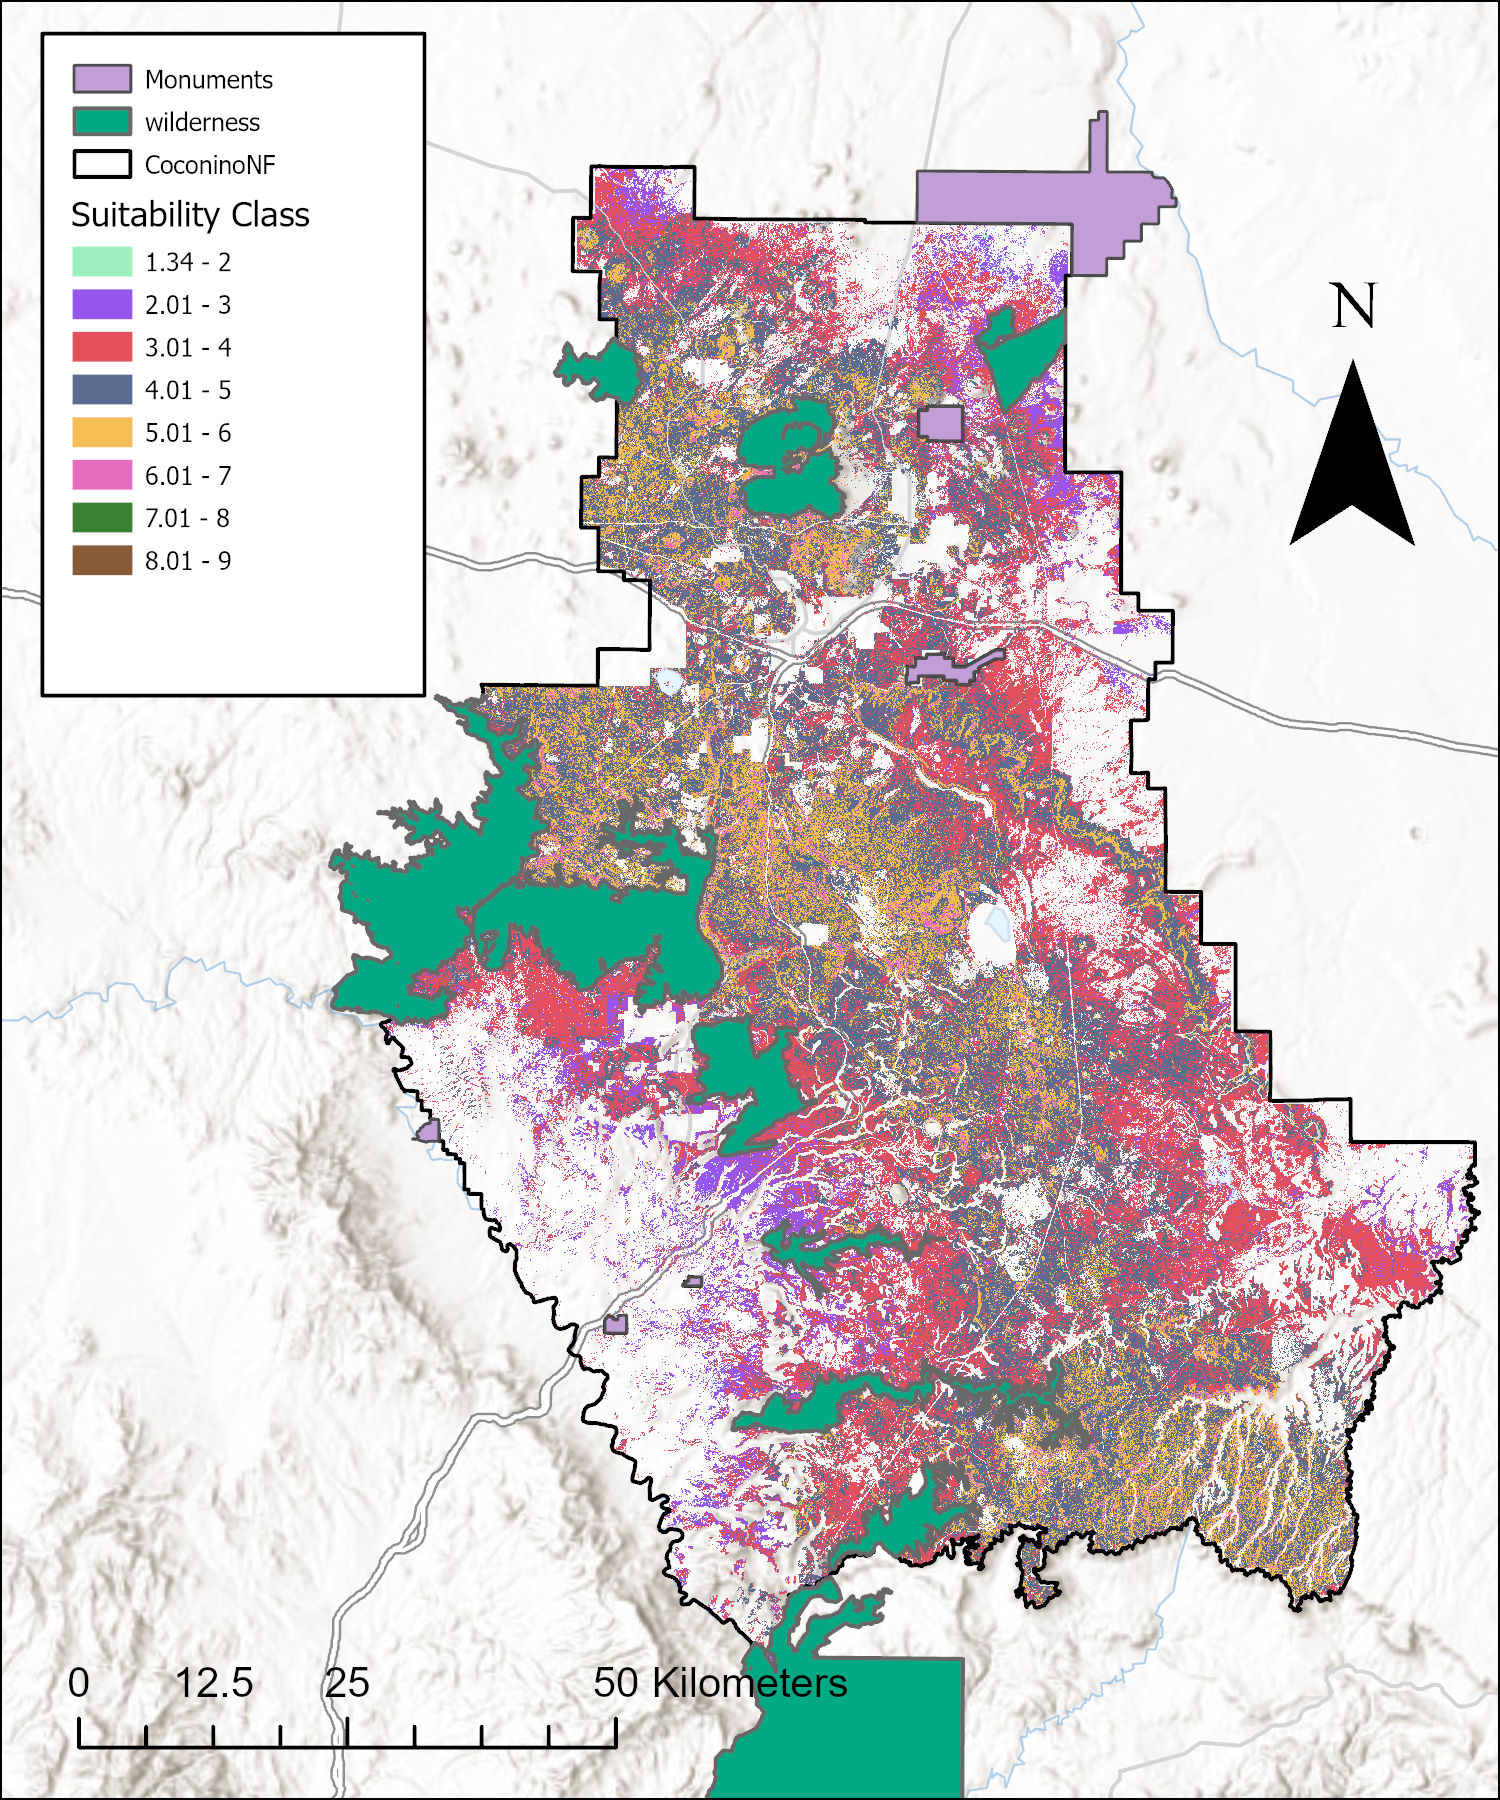
\includegraphics[keepaspectratio]{images/Suitability_map_travis.jpg}}

}

\caption{Suitability Map for Thinning to Enhance Groundwater Recharge}

\end{figure}%

Conclusion

\begin{itemize}
\tightlist
\item
  There are significant portions of the Coconino forest that if thinned,
  are likely to enhance groundwater recharge, however these are not the
  only benefits. While this study was aimed at maximizing recharge,
  these same areas are also likely to reduce wildfire risk and improve
  watershed function enhancing other hydrologic services.
\end{itemize}

Discussion

\begin{itemize}
\item
  novel application of MCDA for mapping areas where forest thinning may
  enhance groundwater recharge.
\item
  It could be adapted to other semi-arid forested
\item
  The Forest Service has a mandate to manage for multiple uses; however,
  groundwater recharge is not currently an explicitly managed use.
  Analyses like these can help identify areas that could be managed with
  aquifer recharge in mind.
\end{itemize}

\section{Future Work}\label{future-work}

\begin{itemize}
\item
  It is important to adjust the suitability map to capture secondary and
  tertiary permeability and porosity in areas underlain by karst. This
  would require improved hydrogeologic mapping of karst surface features
  paired with dye tracing to understand karst flow paths and areas of
  high recharge potential.
\item
  The soil criteria could be refined by mapping soil Hydraulic
  conductivity and field capacity rather than just using soil types
  A---D, providing more detail.
\item
  could be validated with modeling using SWAT or other models
\item
  Paired watershed studies such as those planned in the Lake Mary
  Watershed with groundwater monitoring can be used to validate and
  fine-tune model weighting and decision rules between criteria.
\item
  this methodology could be used across the 2.6 million acres of
  Ponderosa Pine forest in Arizona and New mexico
\item
  State-wide and regional geologic mapping in Arizona is currently only
  at the 1:500,000 scale, more detailed data could improve this type of
  suitability mapping.
\end{itemize}

Acknowledgments

Phasellus interdum tincidunt ex, a euismod massa pulvinar at. Ut
fringilla ut nisi nec volutpat. Morbi imperdiet congue tincidunt.
Vivamus eget rutrum purus. Etiam et pretium justo. Donec et egestas sem.
Donec molestie ex sit amet viverra egestas. Nullam justo nulla,
fringilla at iaculis in, posuere non mauris. Ut eget imperdiet elit.

Open research

Phasellus interdum tincidunt ex, a euismod massa pulvinar at. Ut
fringilla ut nisi nec volutpat. Morbi imperdiet congue tincidunt.
Vivamus eget rutrum purus. Etiam et pretium justo. Donec et egestas sem.
Donec molestie ex sit amet viverra egestas. Nullam justo nulla,
fringilla at iaculis in, posuere non mauris. Ut eget imperdiet elit.

References

\renewcommand{\bibsection}{}
\bibliography{bibliography.bib}





\end{document}
